\documentclass[Supplementary.tex]{subfiles}
\begin{document}
 \begin{figure}[ht]
     \centering
     \begin{subfigure}{0.3\textwidth}
        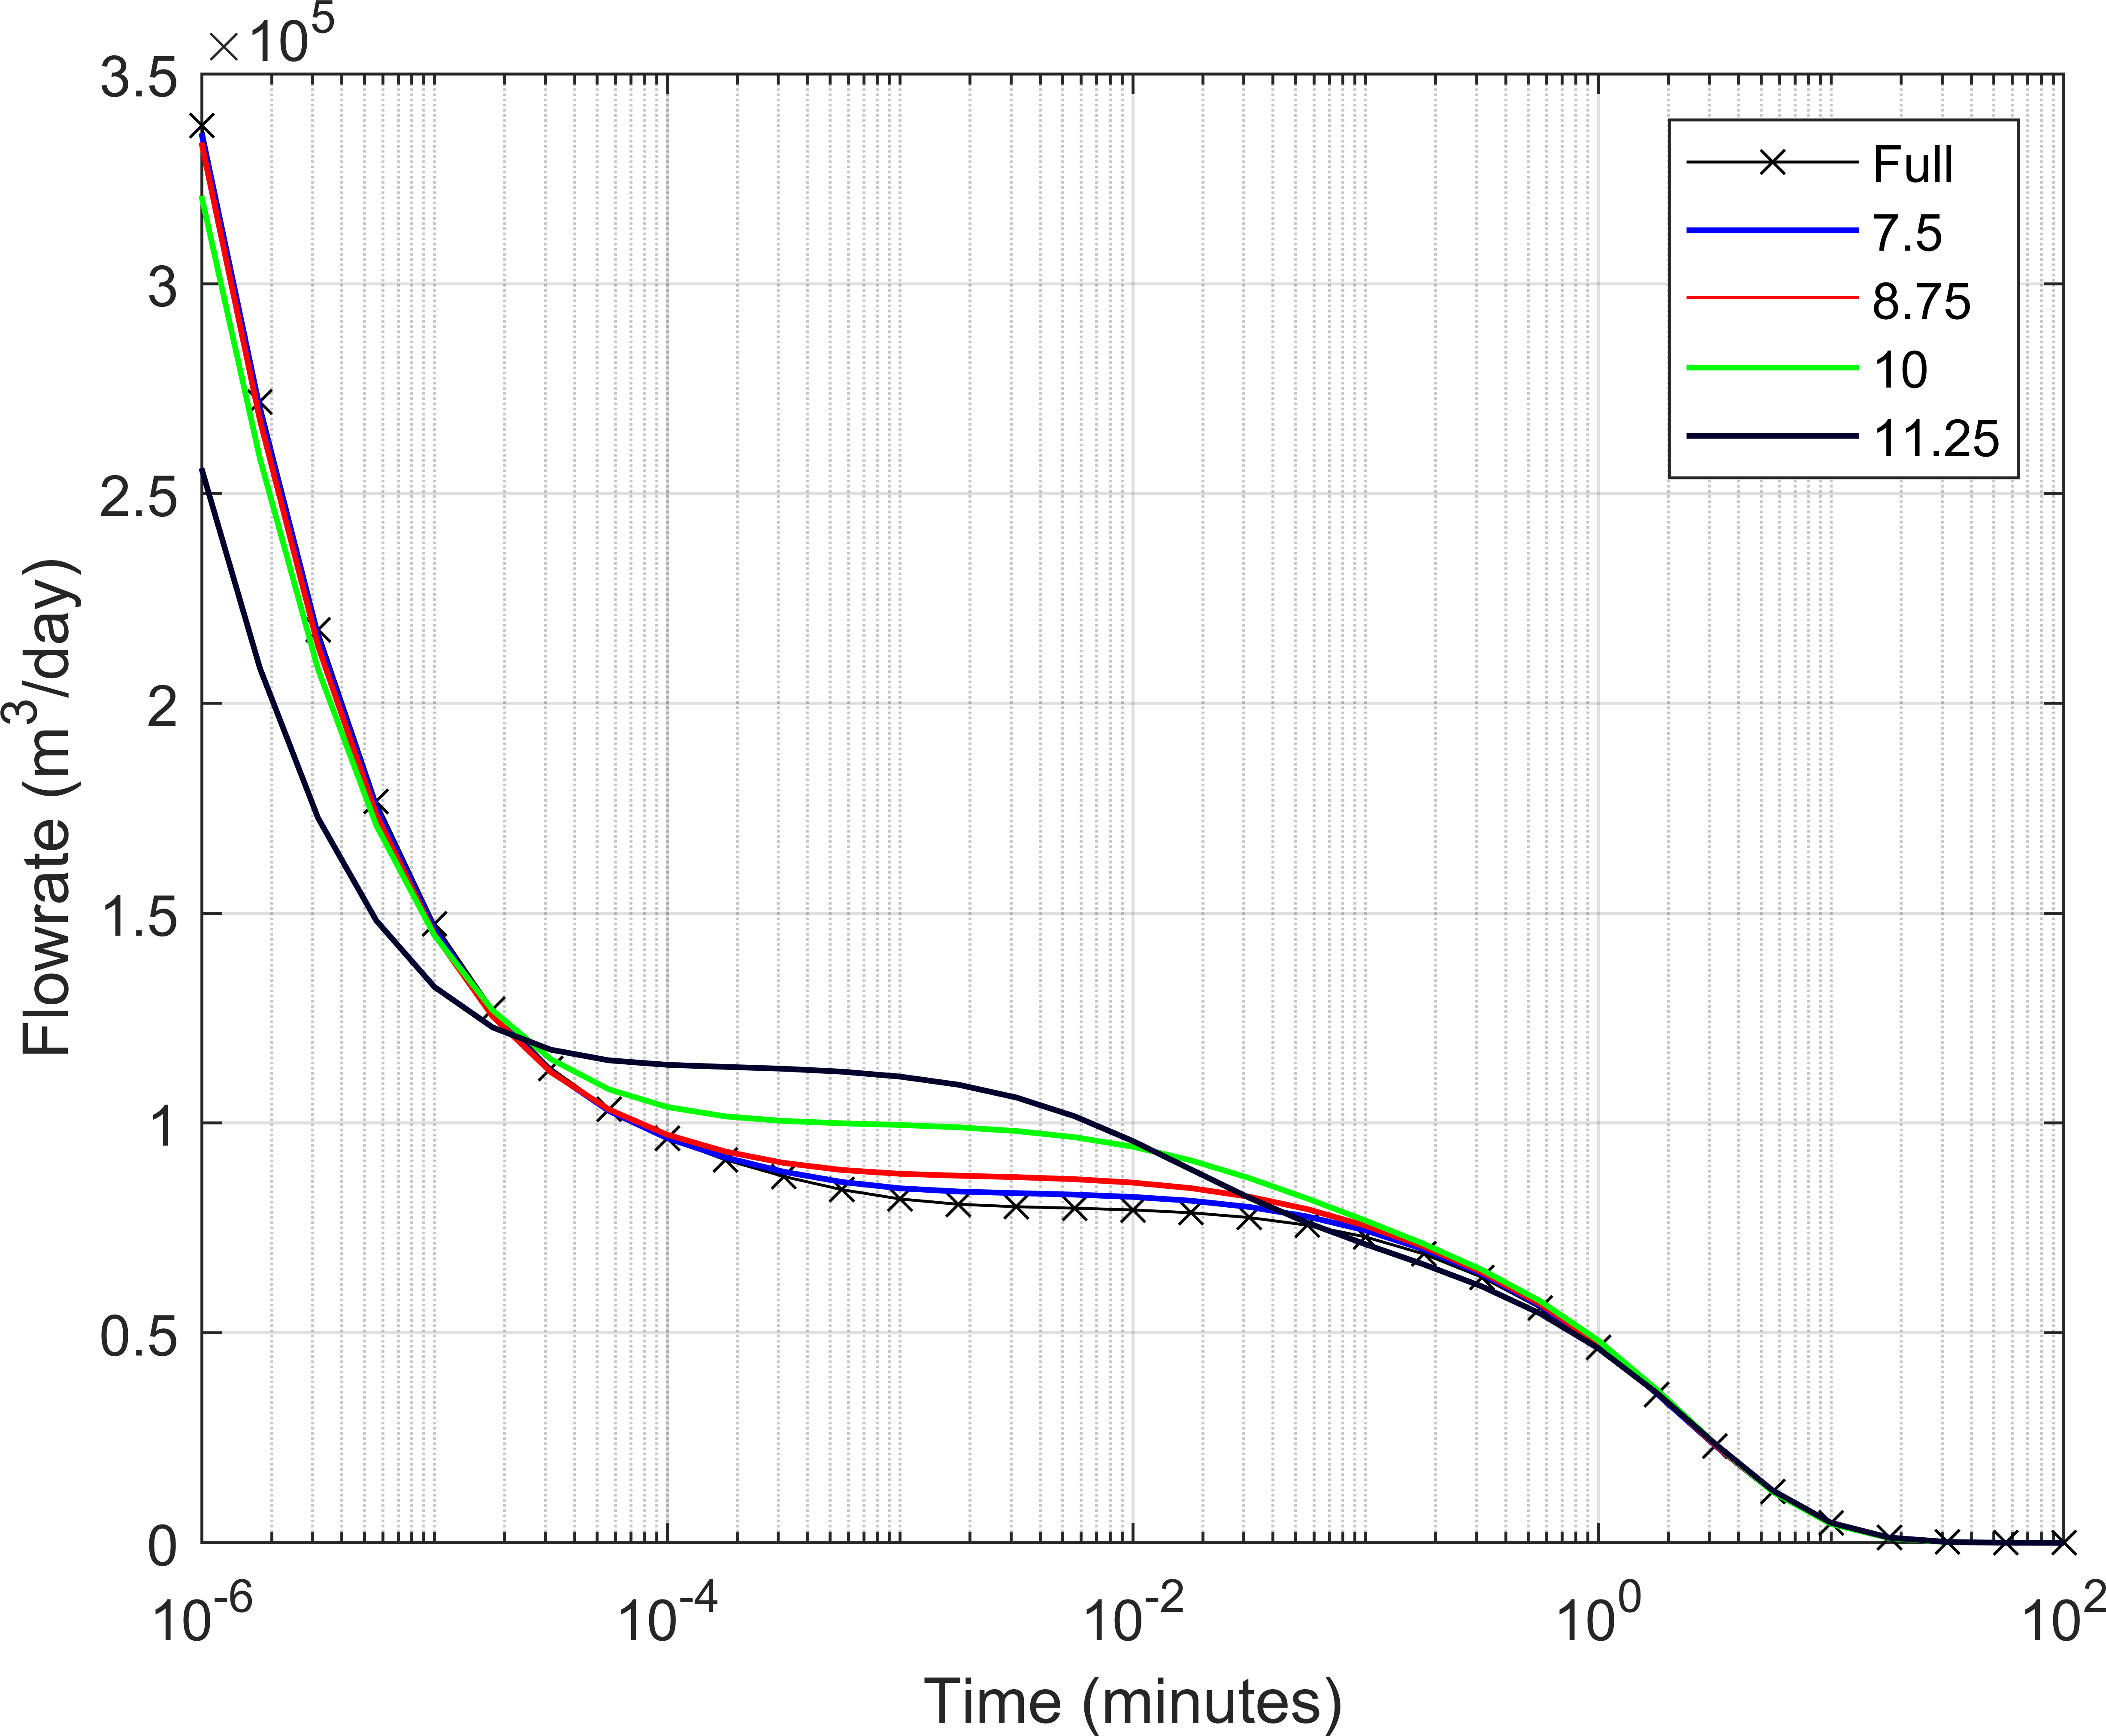
\includegraphics[width=\textwidth]{3D_DD/Plot_Drawdown_Case_01_nohead.png}
        \subcaption{Case 1}
        \label{fig:3D_DD_1}
     \end{subfigure}
     \begin{subfigure}{0.3\textwidth}
        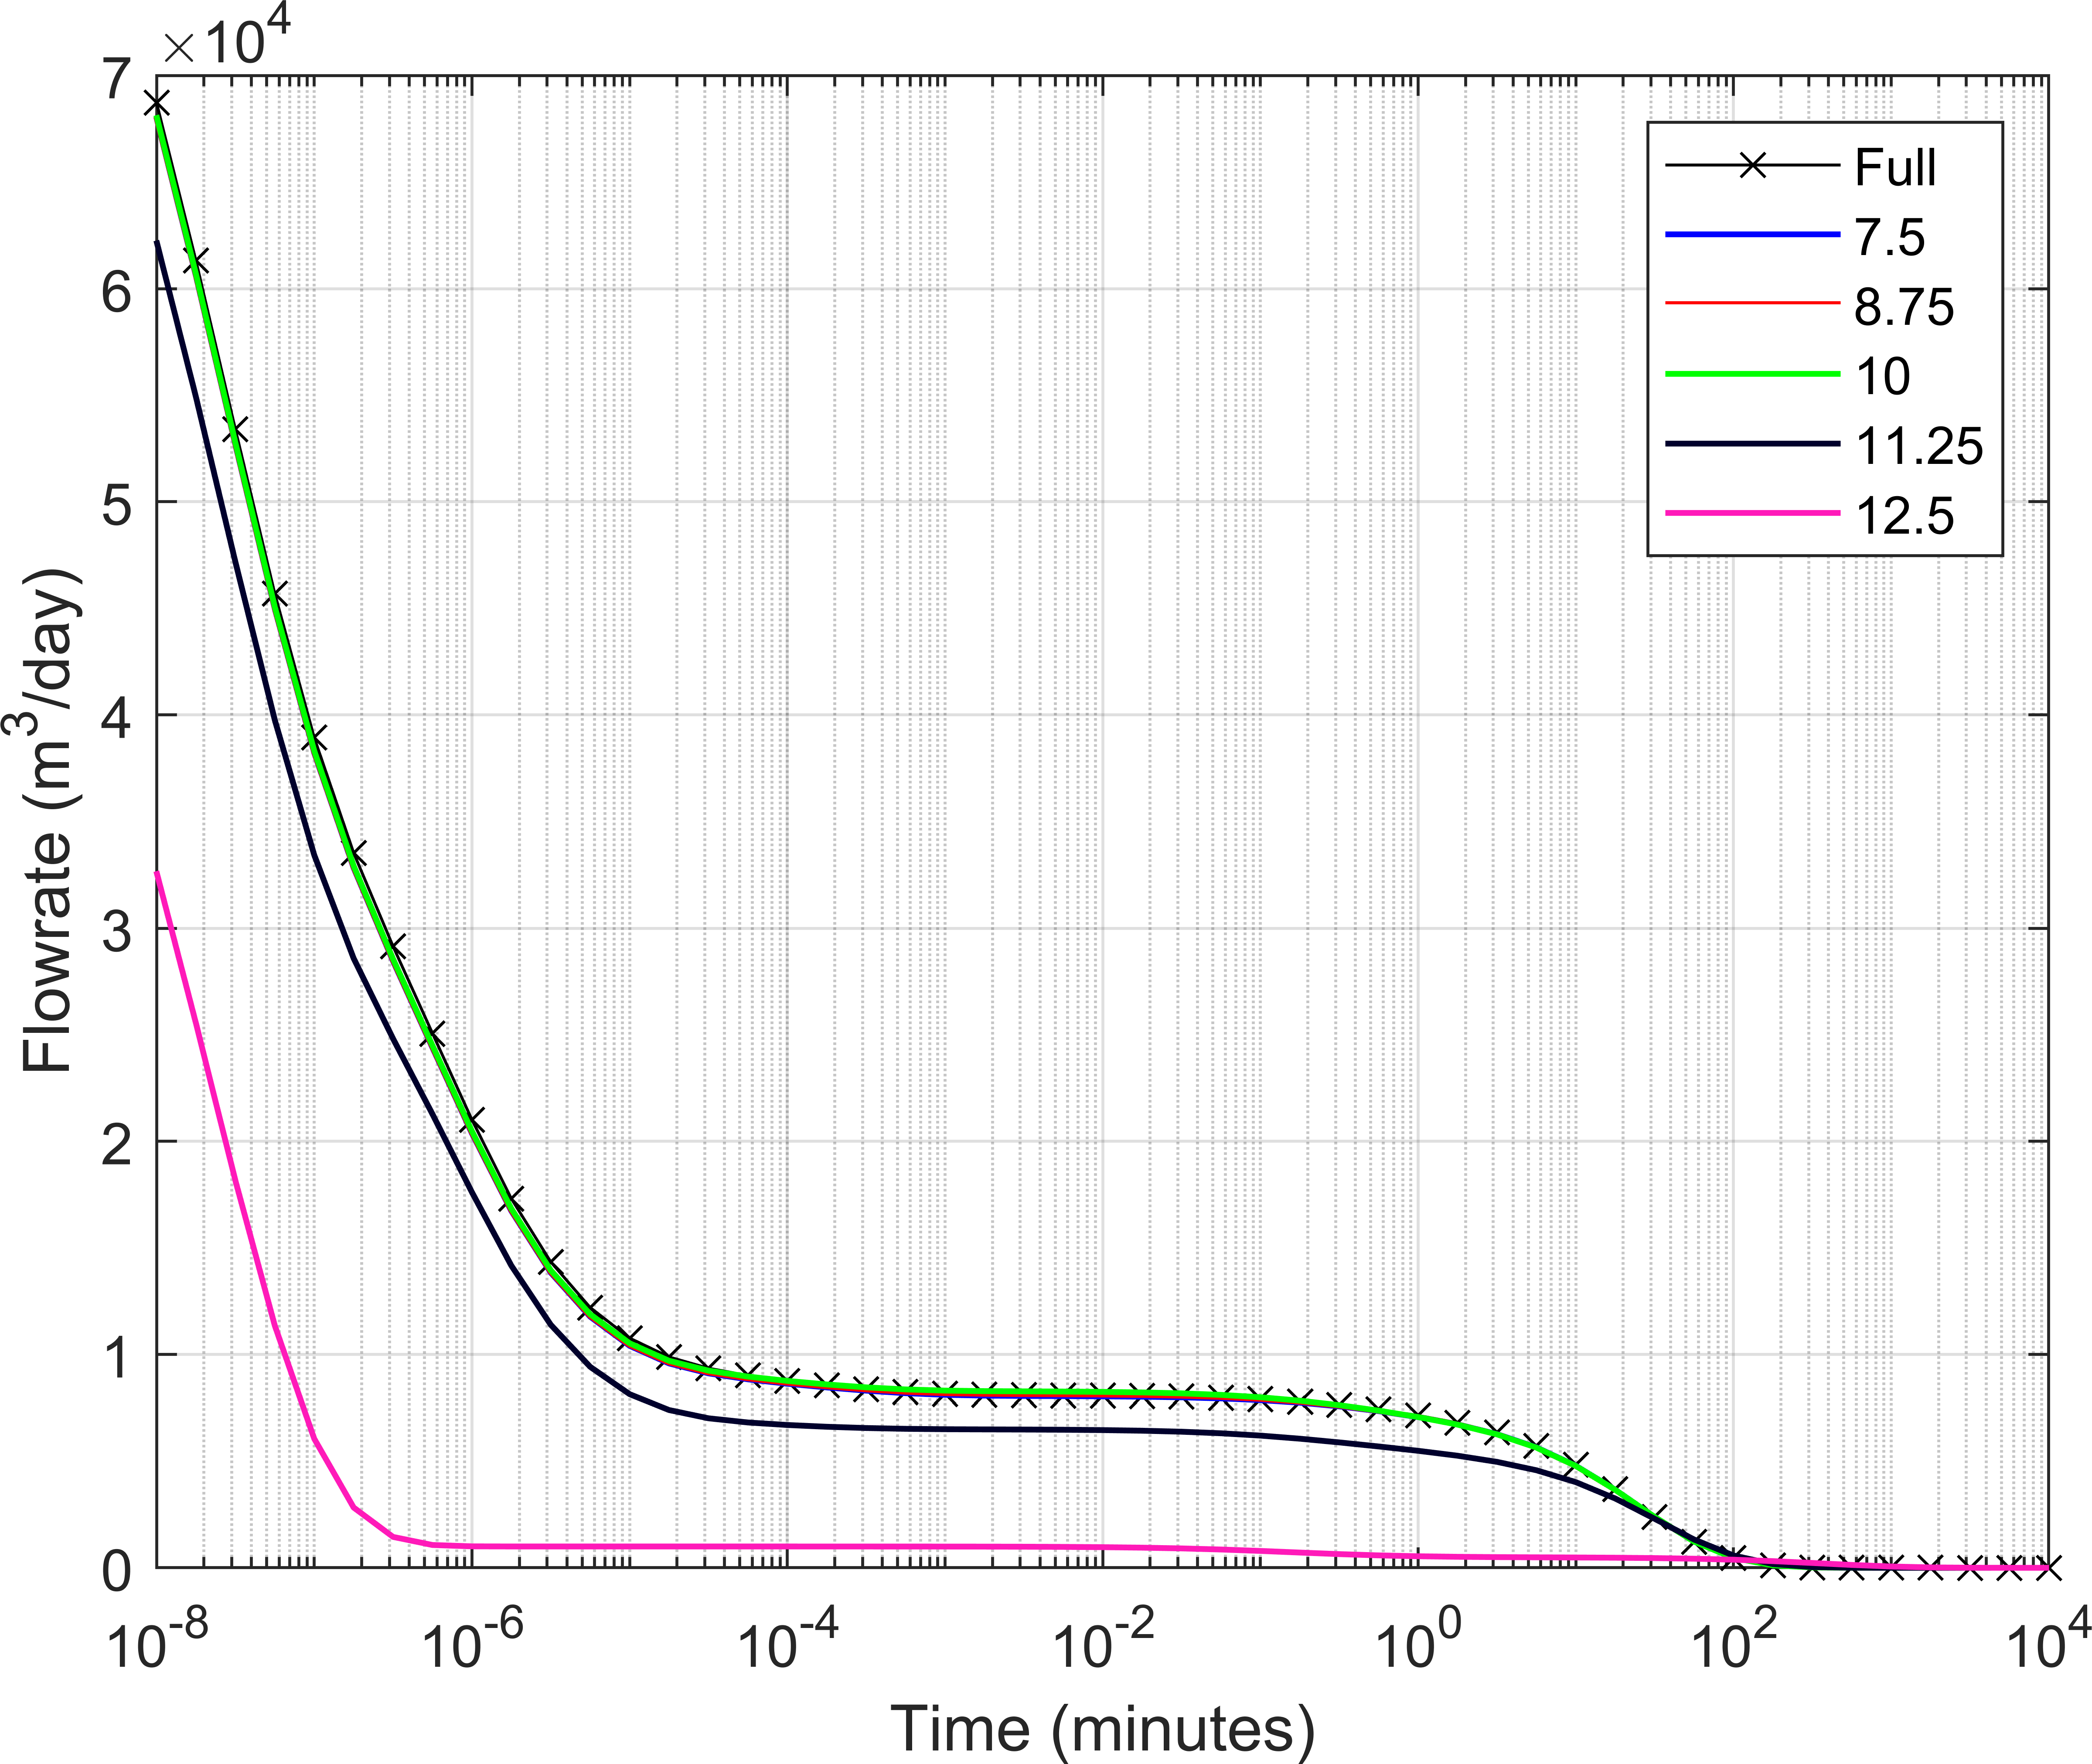
\includegraphics[width=\textwidth]{3D_DD/Plot_Drawdown_Case_02_nohead.png}
        \subcaption{Case 2}
        \label{fig:3D_DD_2}
     \end{subfigure}
     \begin{subfigure}{0.3\textwidth}
        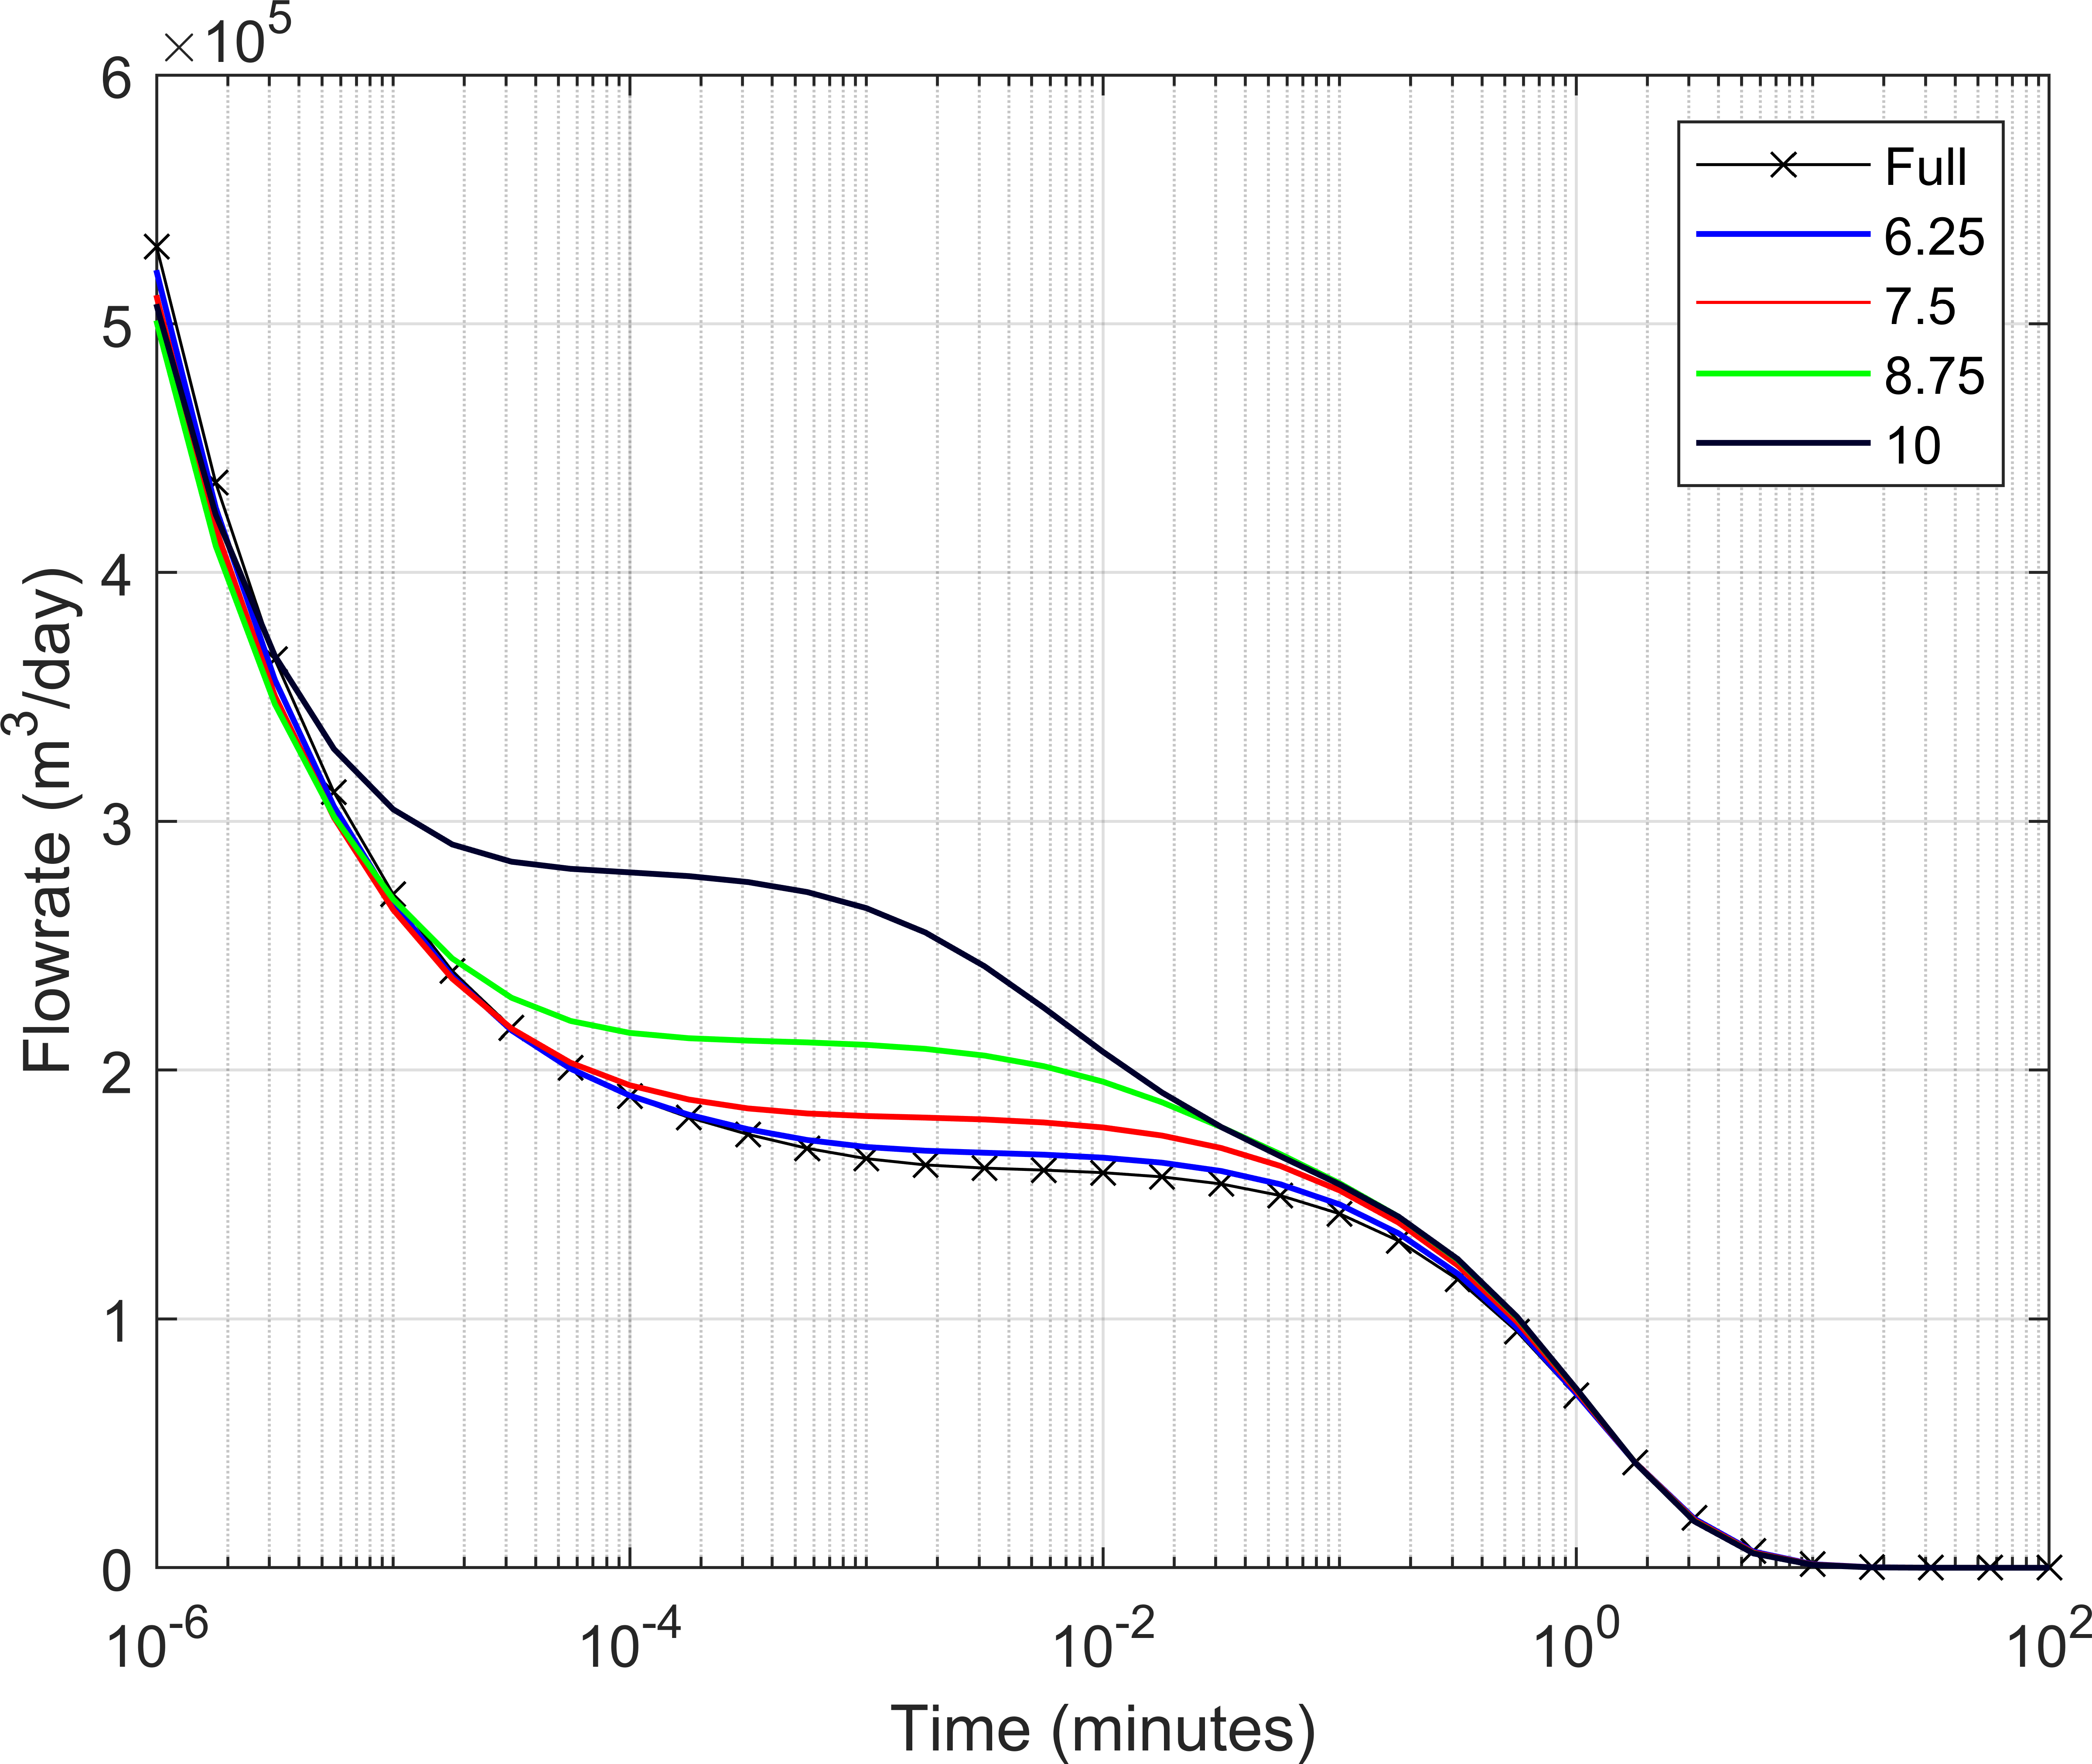
\includegraphics[width=\textwidth]{3D_DD/Plot_Drawdown_Case_03_nohead.png}
        \subcaption{Case 3}
        \label{fig:3D_DD_3}
     \end{subfigure}
     \\
     \begin{subfigure}{0.3\textwidth}
        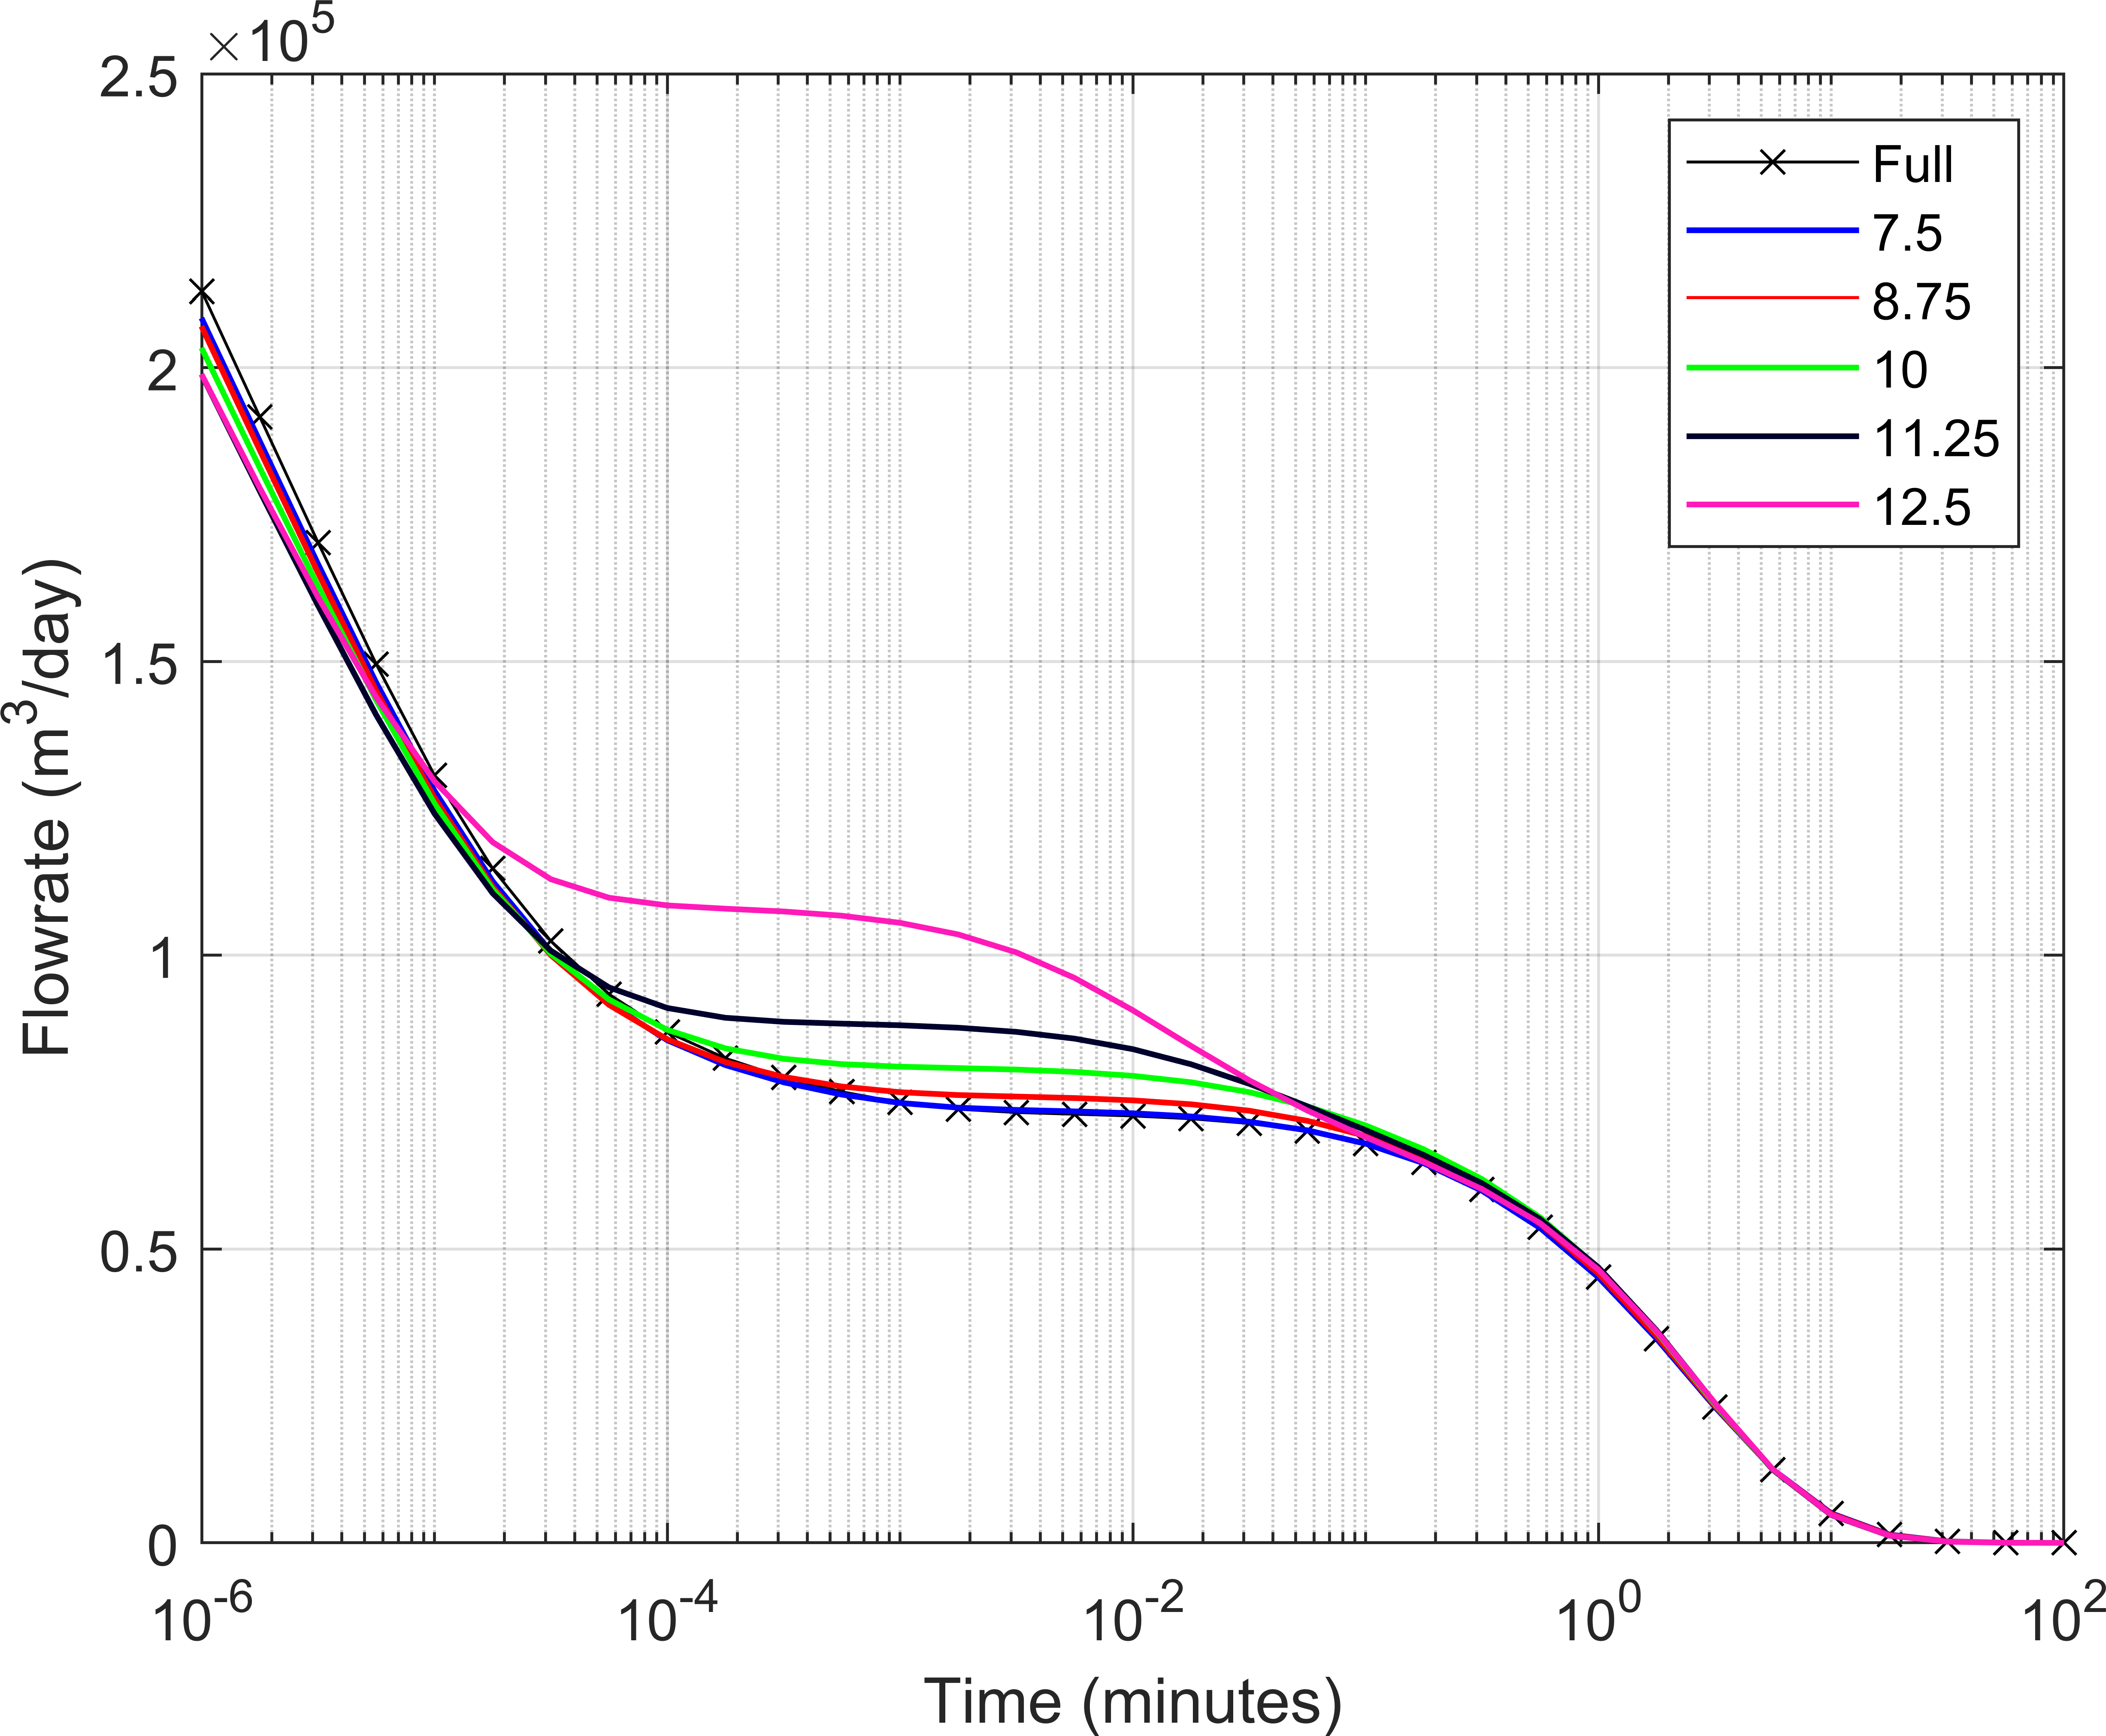
\includegraphics[width=\textwidth]{3D_DD/Plot_Drawdown_Case_04_nohead.png}
        \subcaption{Case 4}
        \label{fig:3D_DD_4}
     \end{subfigure}
     \begin{subfigure}{0.3\textwidth}
        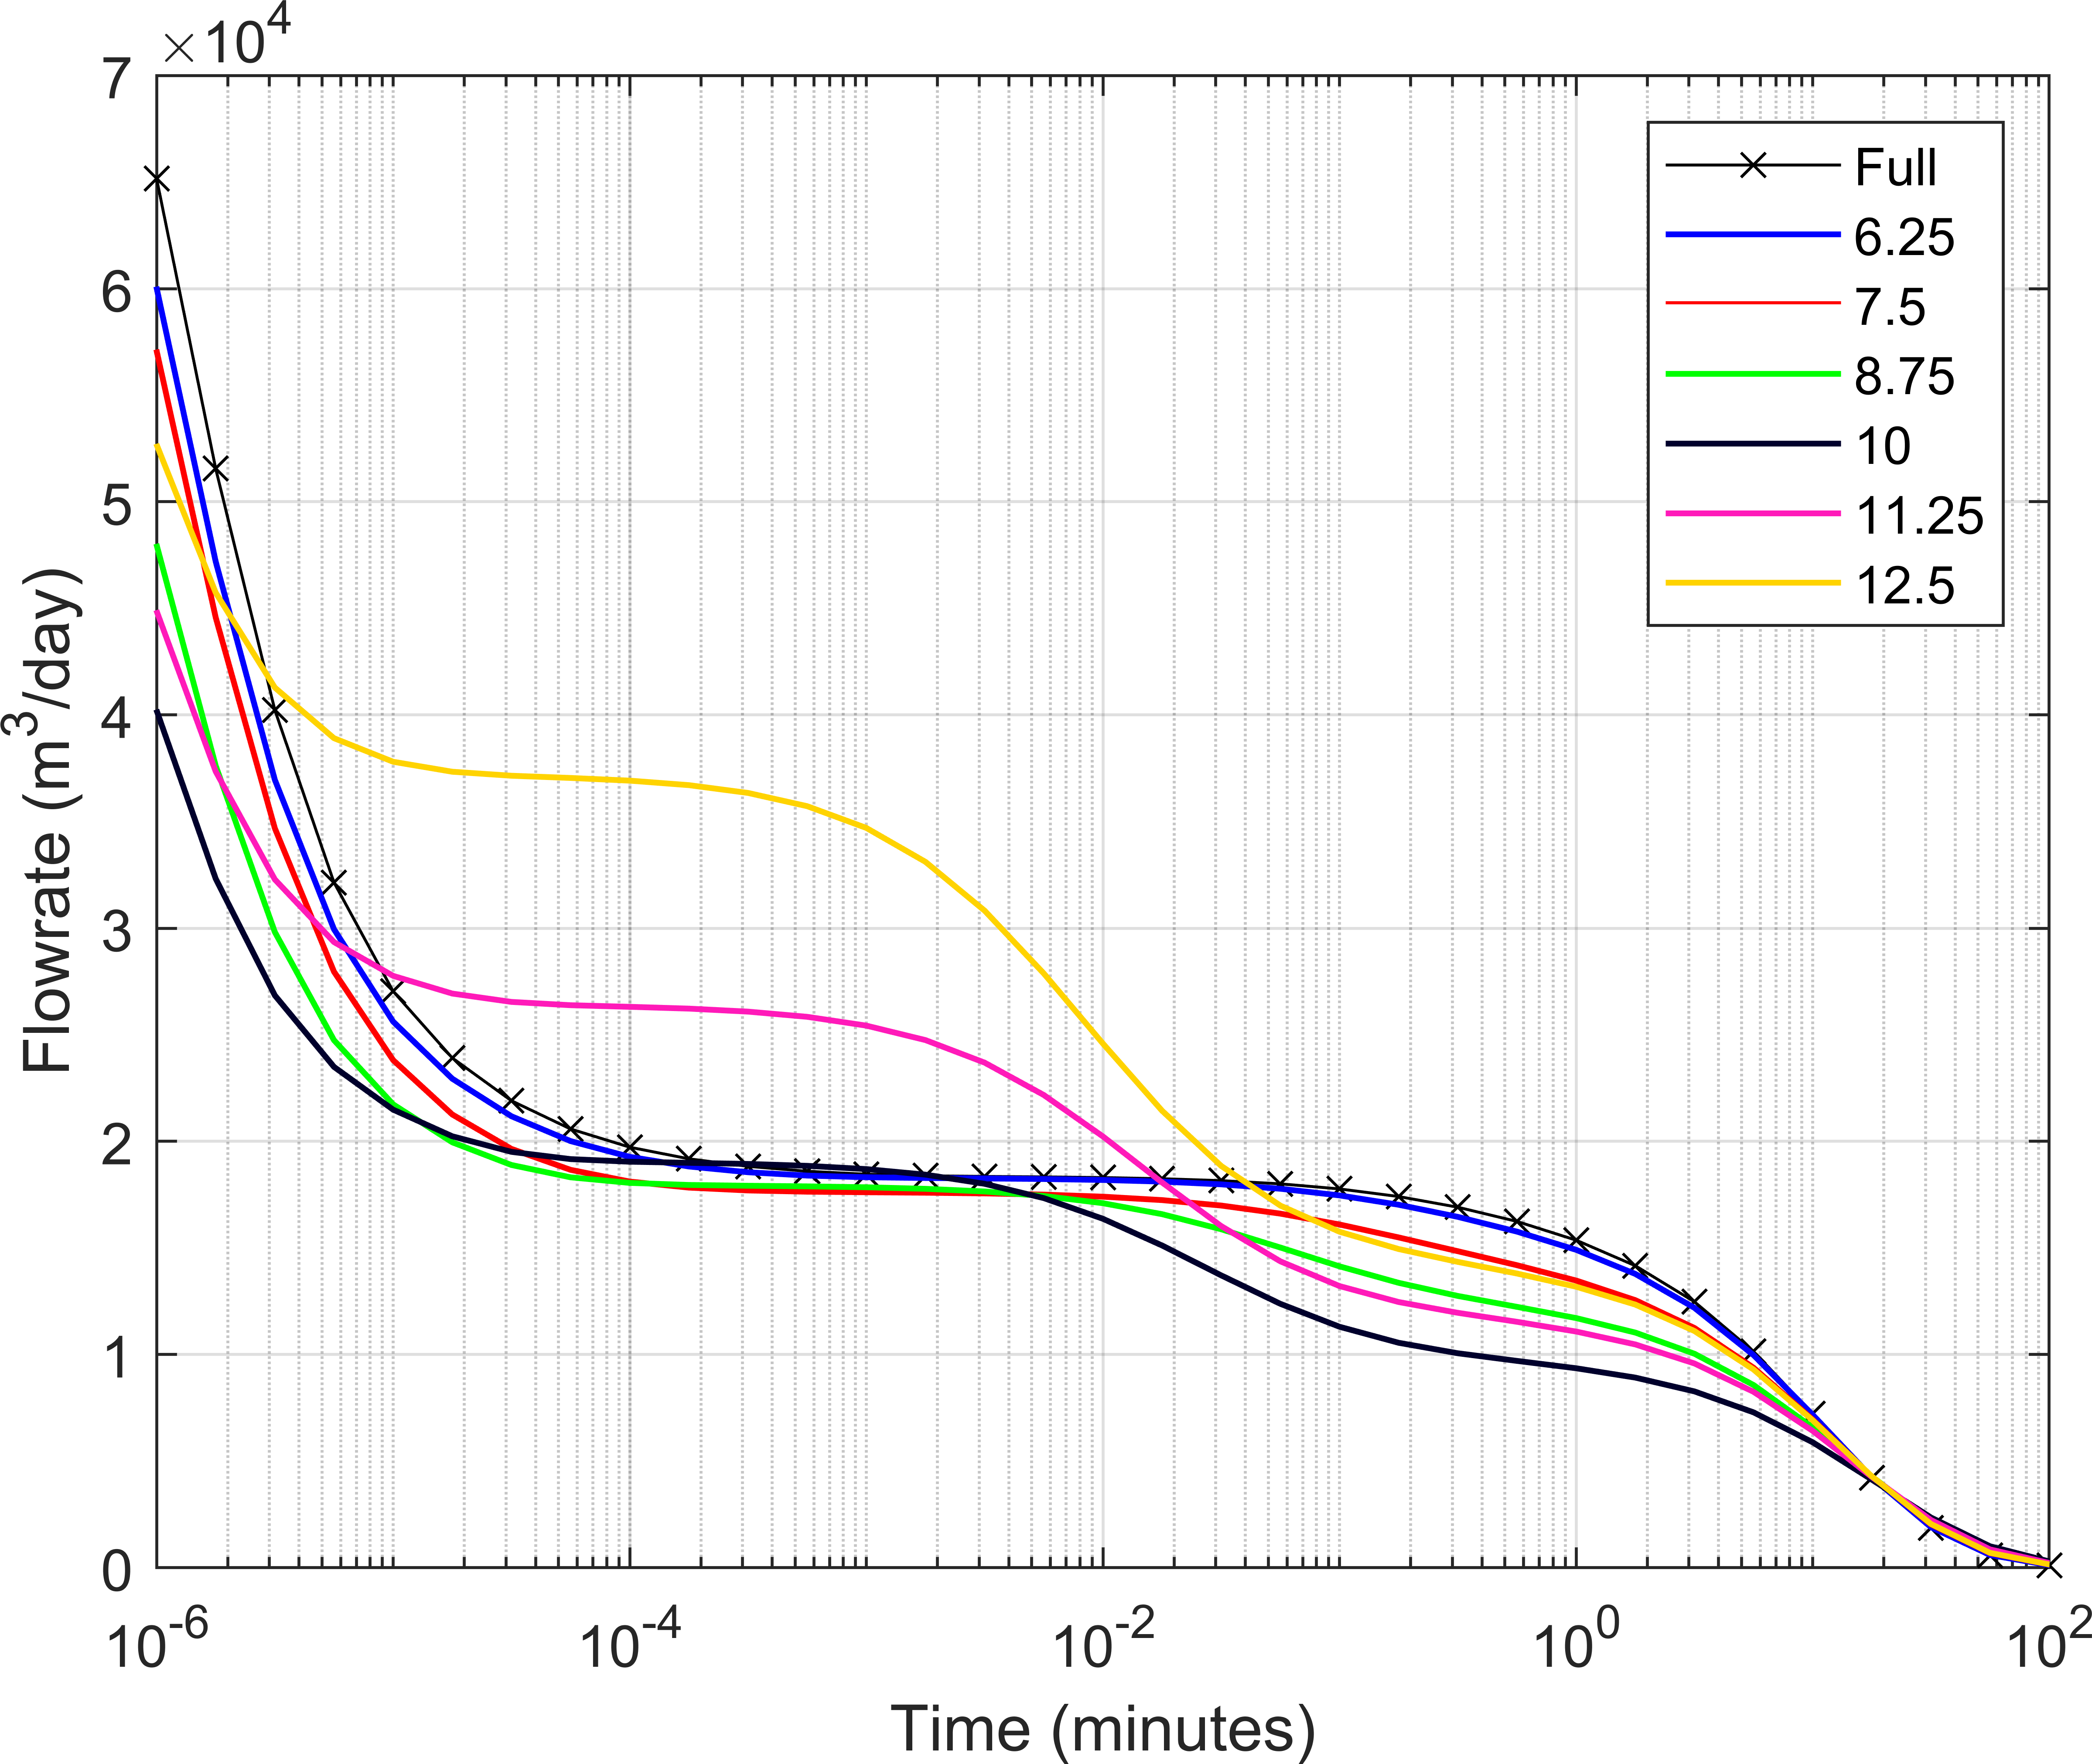
\includegraphics[width=\textwidth]{3D_DD/Plot_Drawdown_Case_05_nohead.png}
        \subcaption{Case 5}
        \label{fig:3D_DD_5}
     \end{subfigure}
     \begin{subfigure}{0.3\textwidth}
        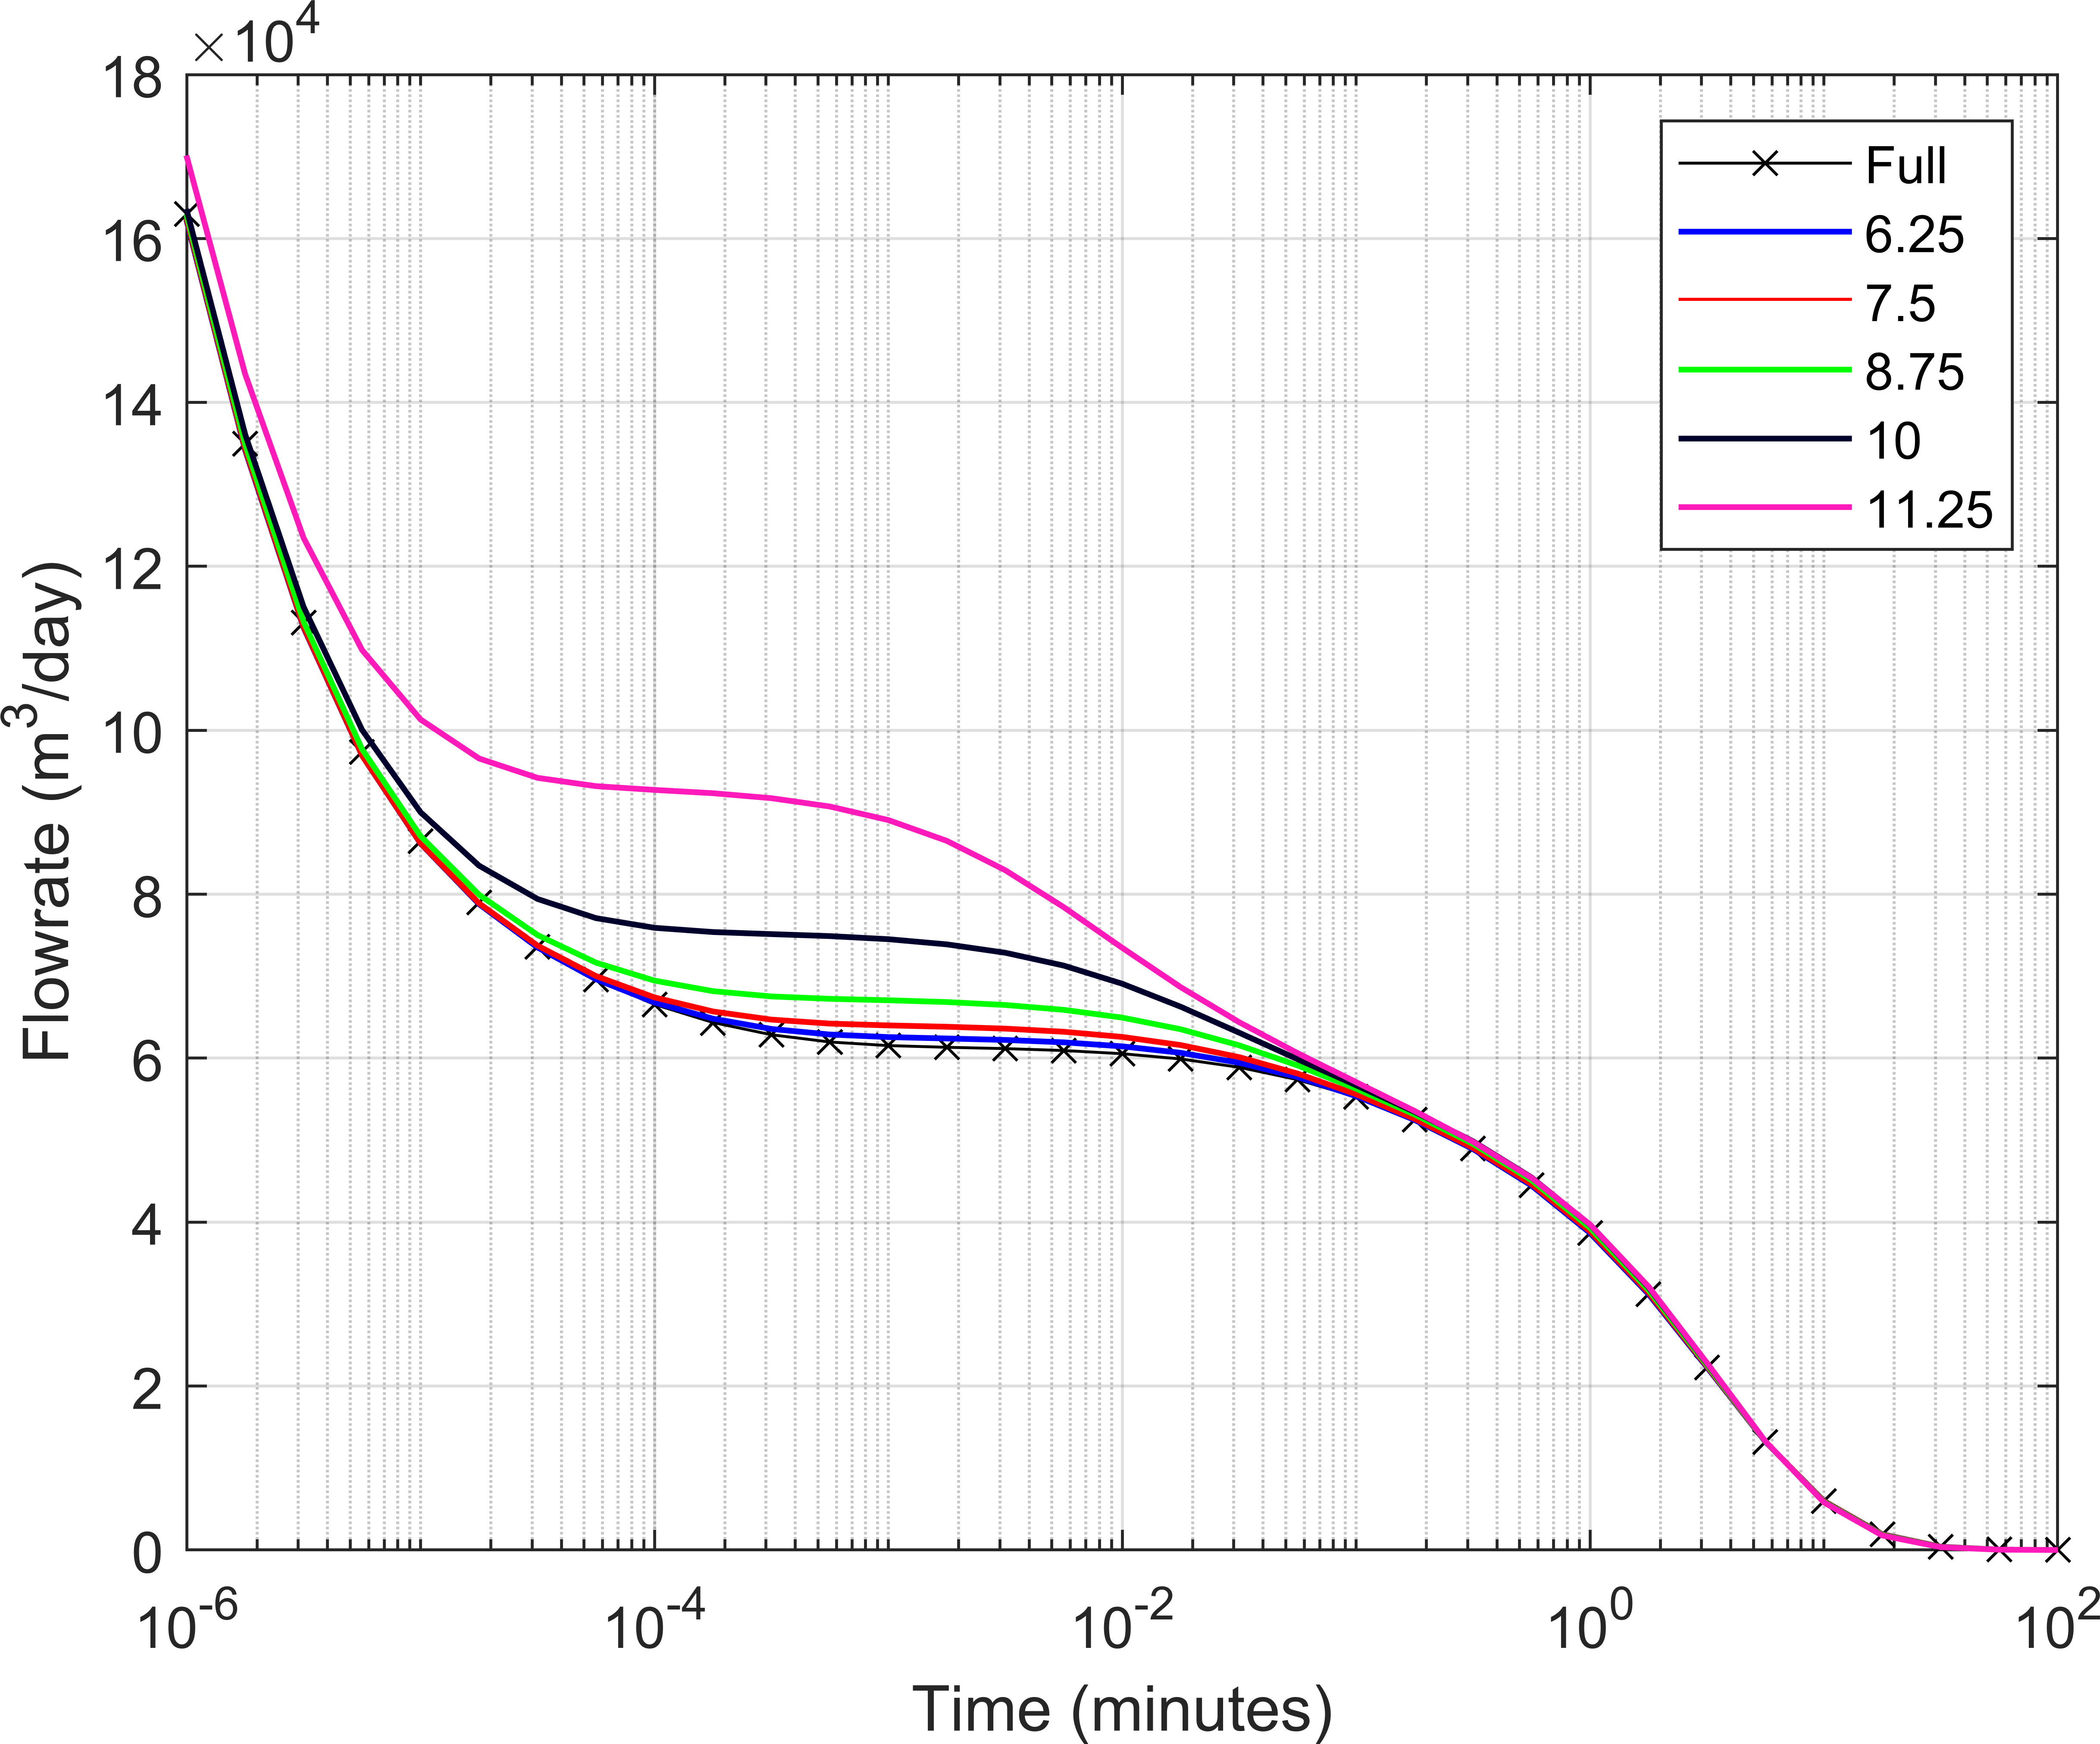
\includegraphics[width=\textwidth]{3D_DD/Plot_Drawdown_Case_06_nohead.png}
        \subcaption{Case 6}
        \label{fig:3D_DD_6}
     \end{subfigure}
     \\
     \begin{subfigure}{0.3\textwidth}
        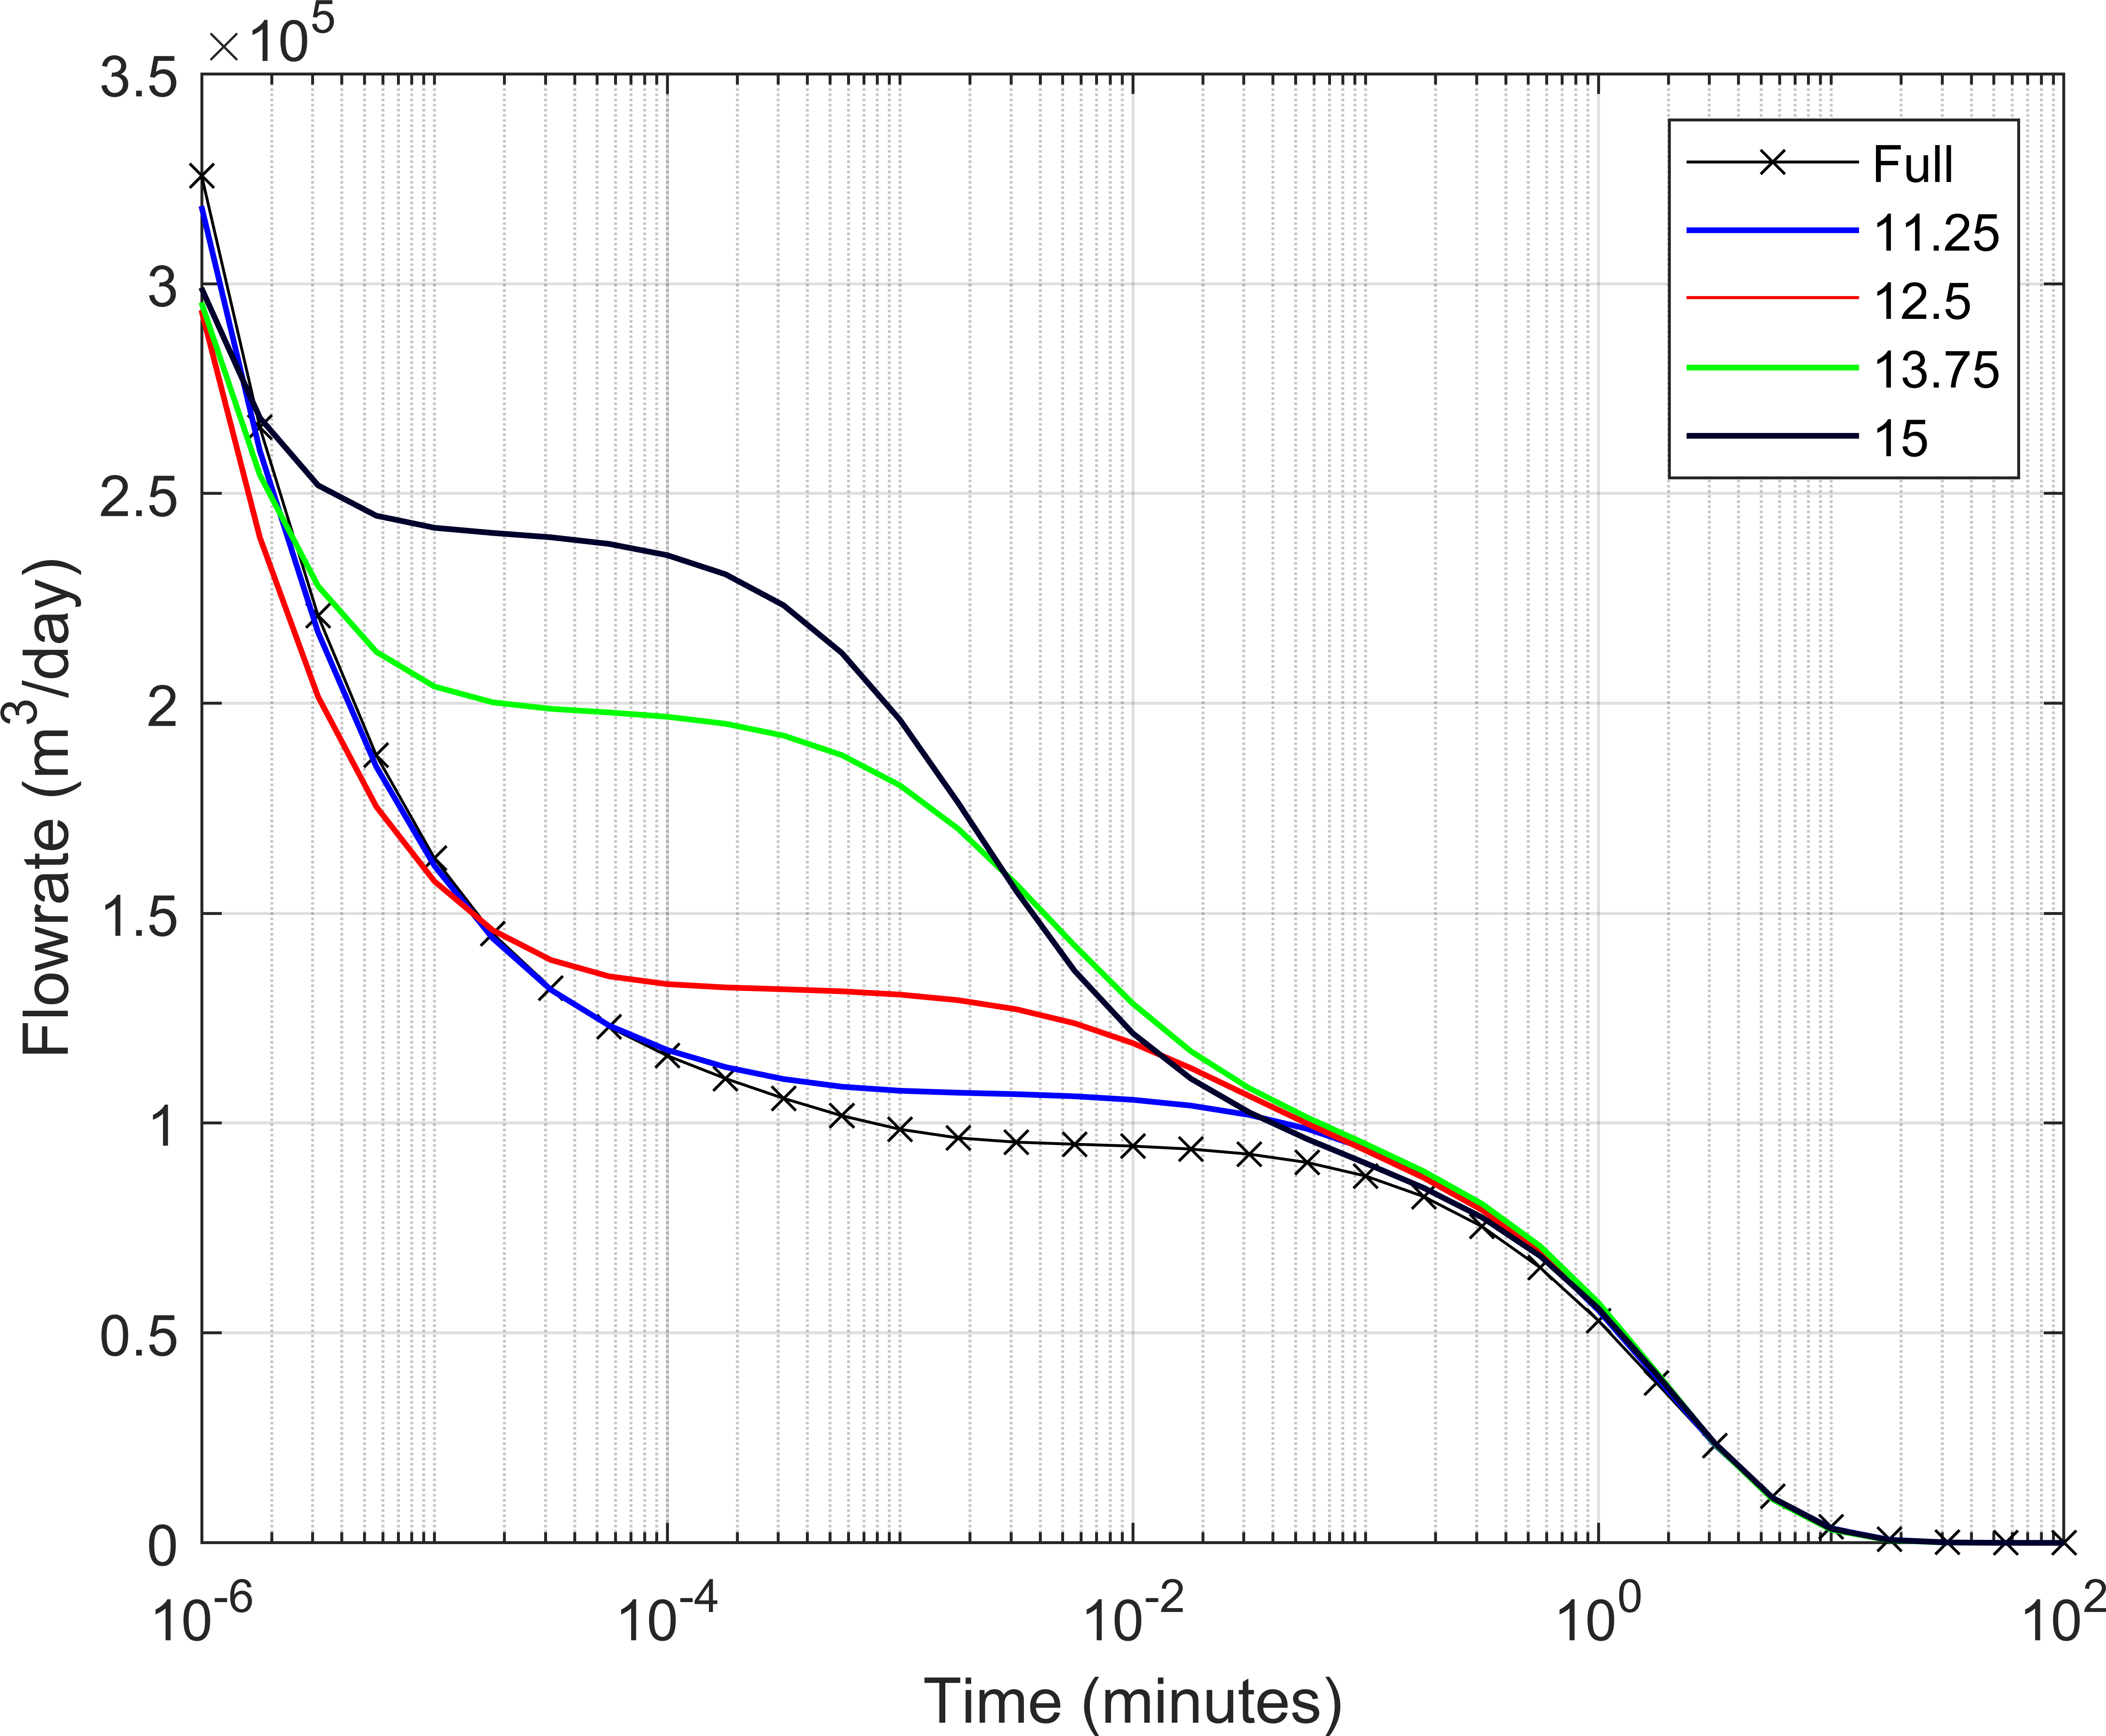
\includegraphics[width=\textwidth]{3D_DD/Plot_Drawdown_Case_07_nohead.png}
        \subcaption{Case 7}
        \label{fig:3D_DD_7}
     \end{subfigure}
     \begin{subfigure}{0.3\textwidth}
        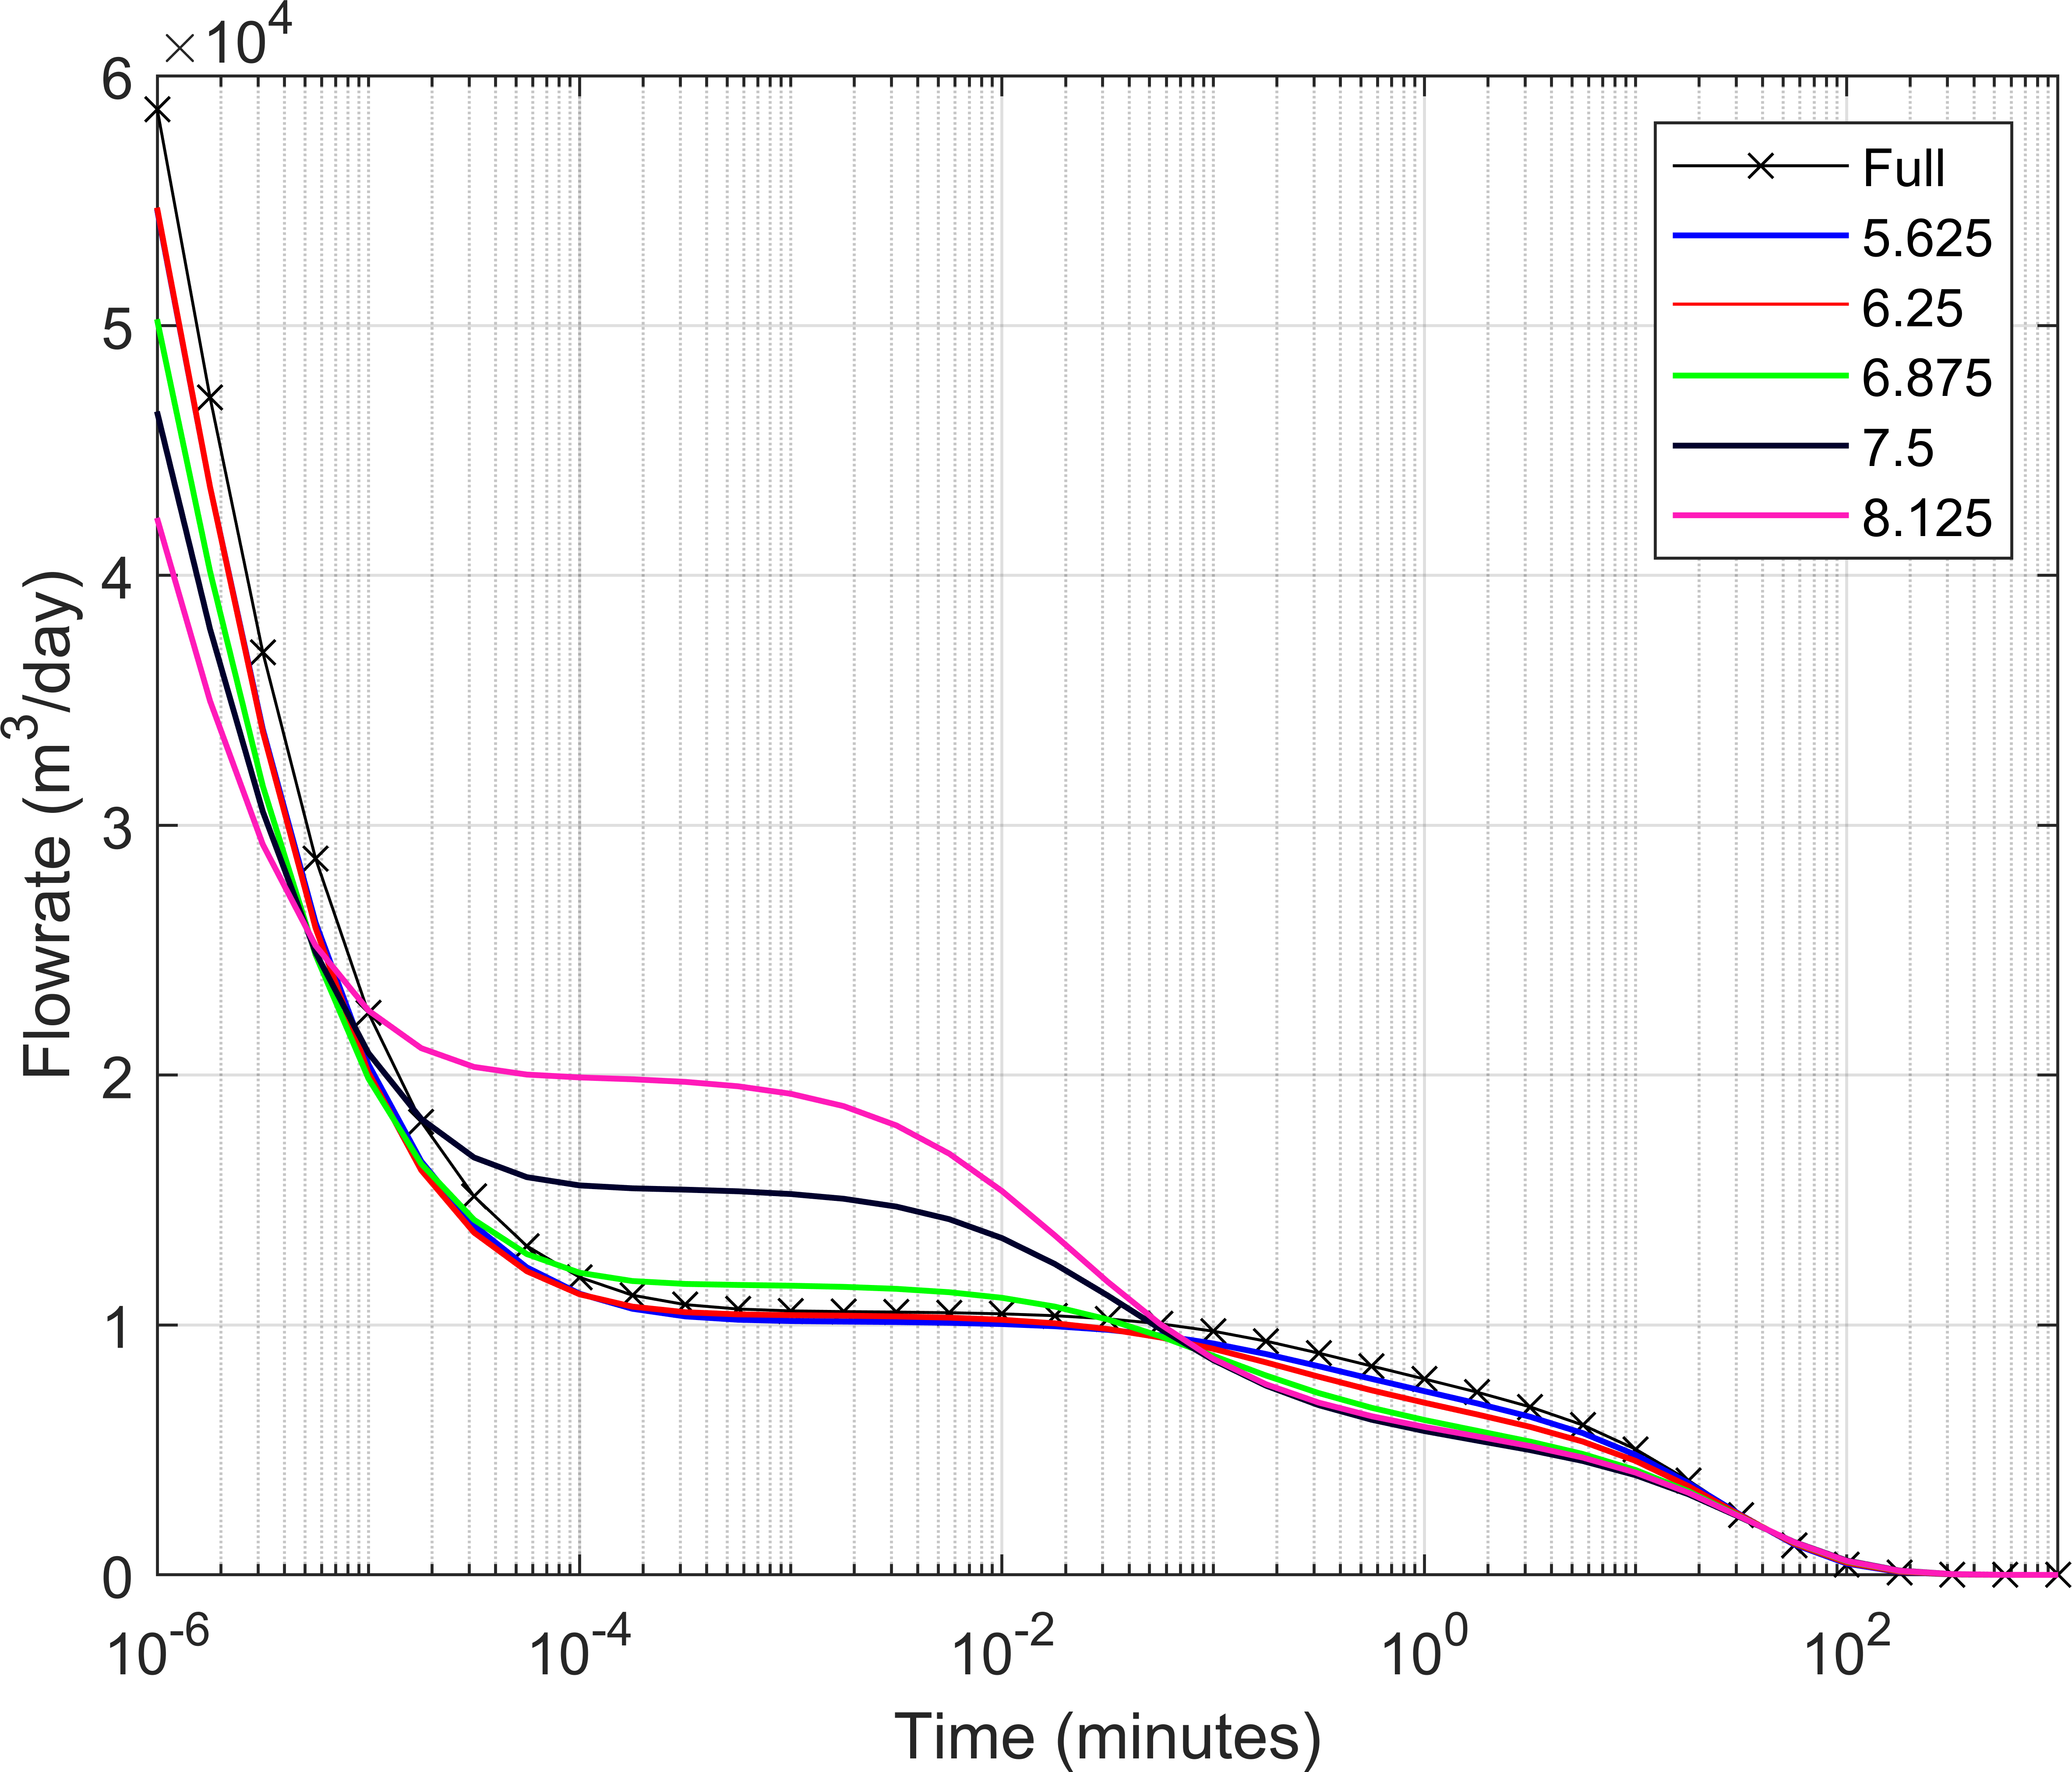
\includegraphics[width=\textwidth]{3D_DD/Plot_Drawdown_Case_08_nohead.png}
        \subcaption{Case 8}
        \label{fig:3D_DD_8}
     \end{subfigure}
     \begin{subfigure}{0.3\textwidth}
        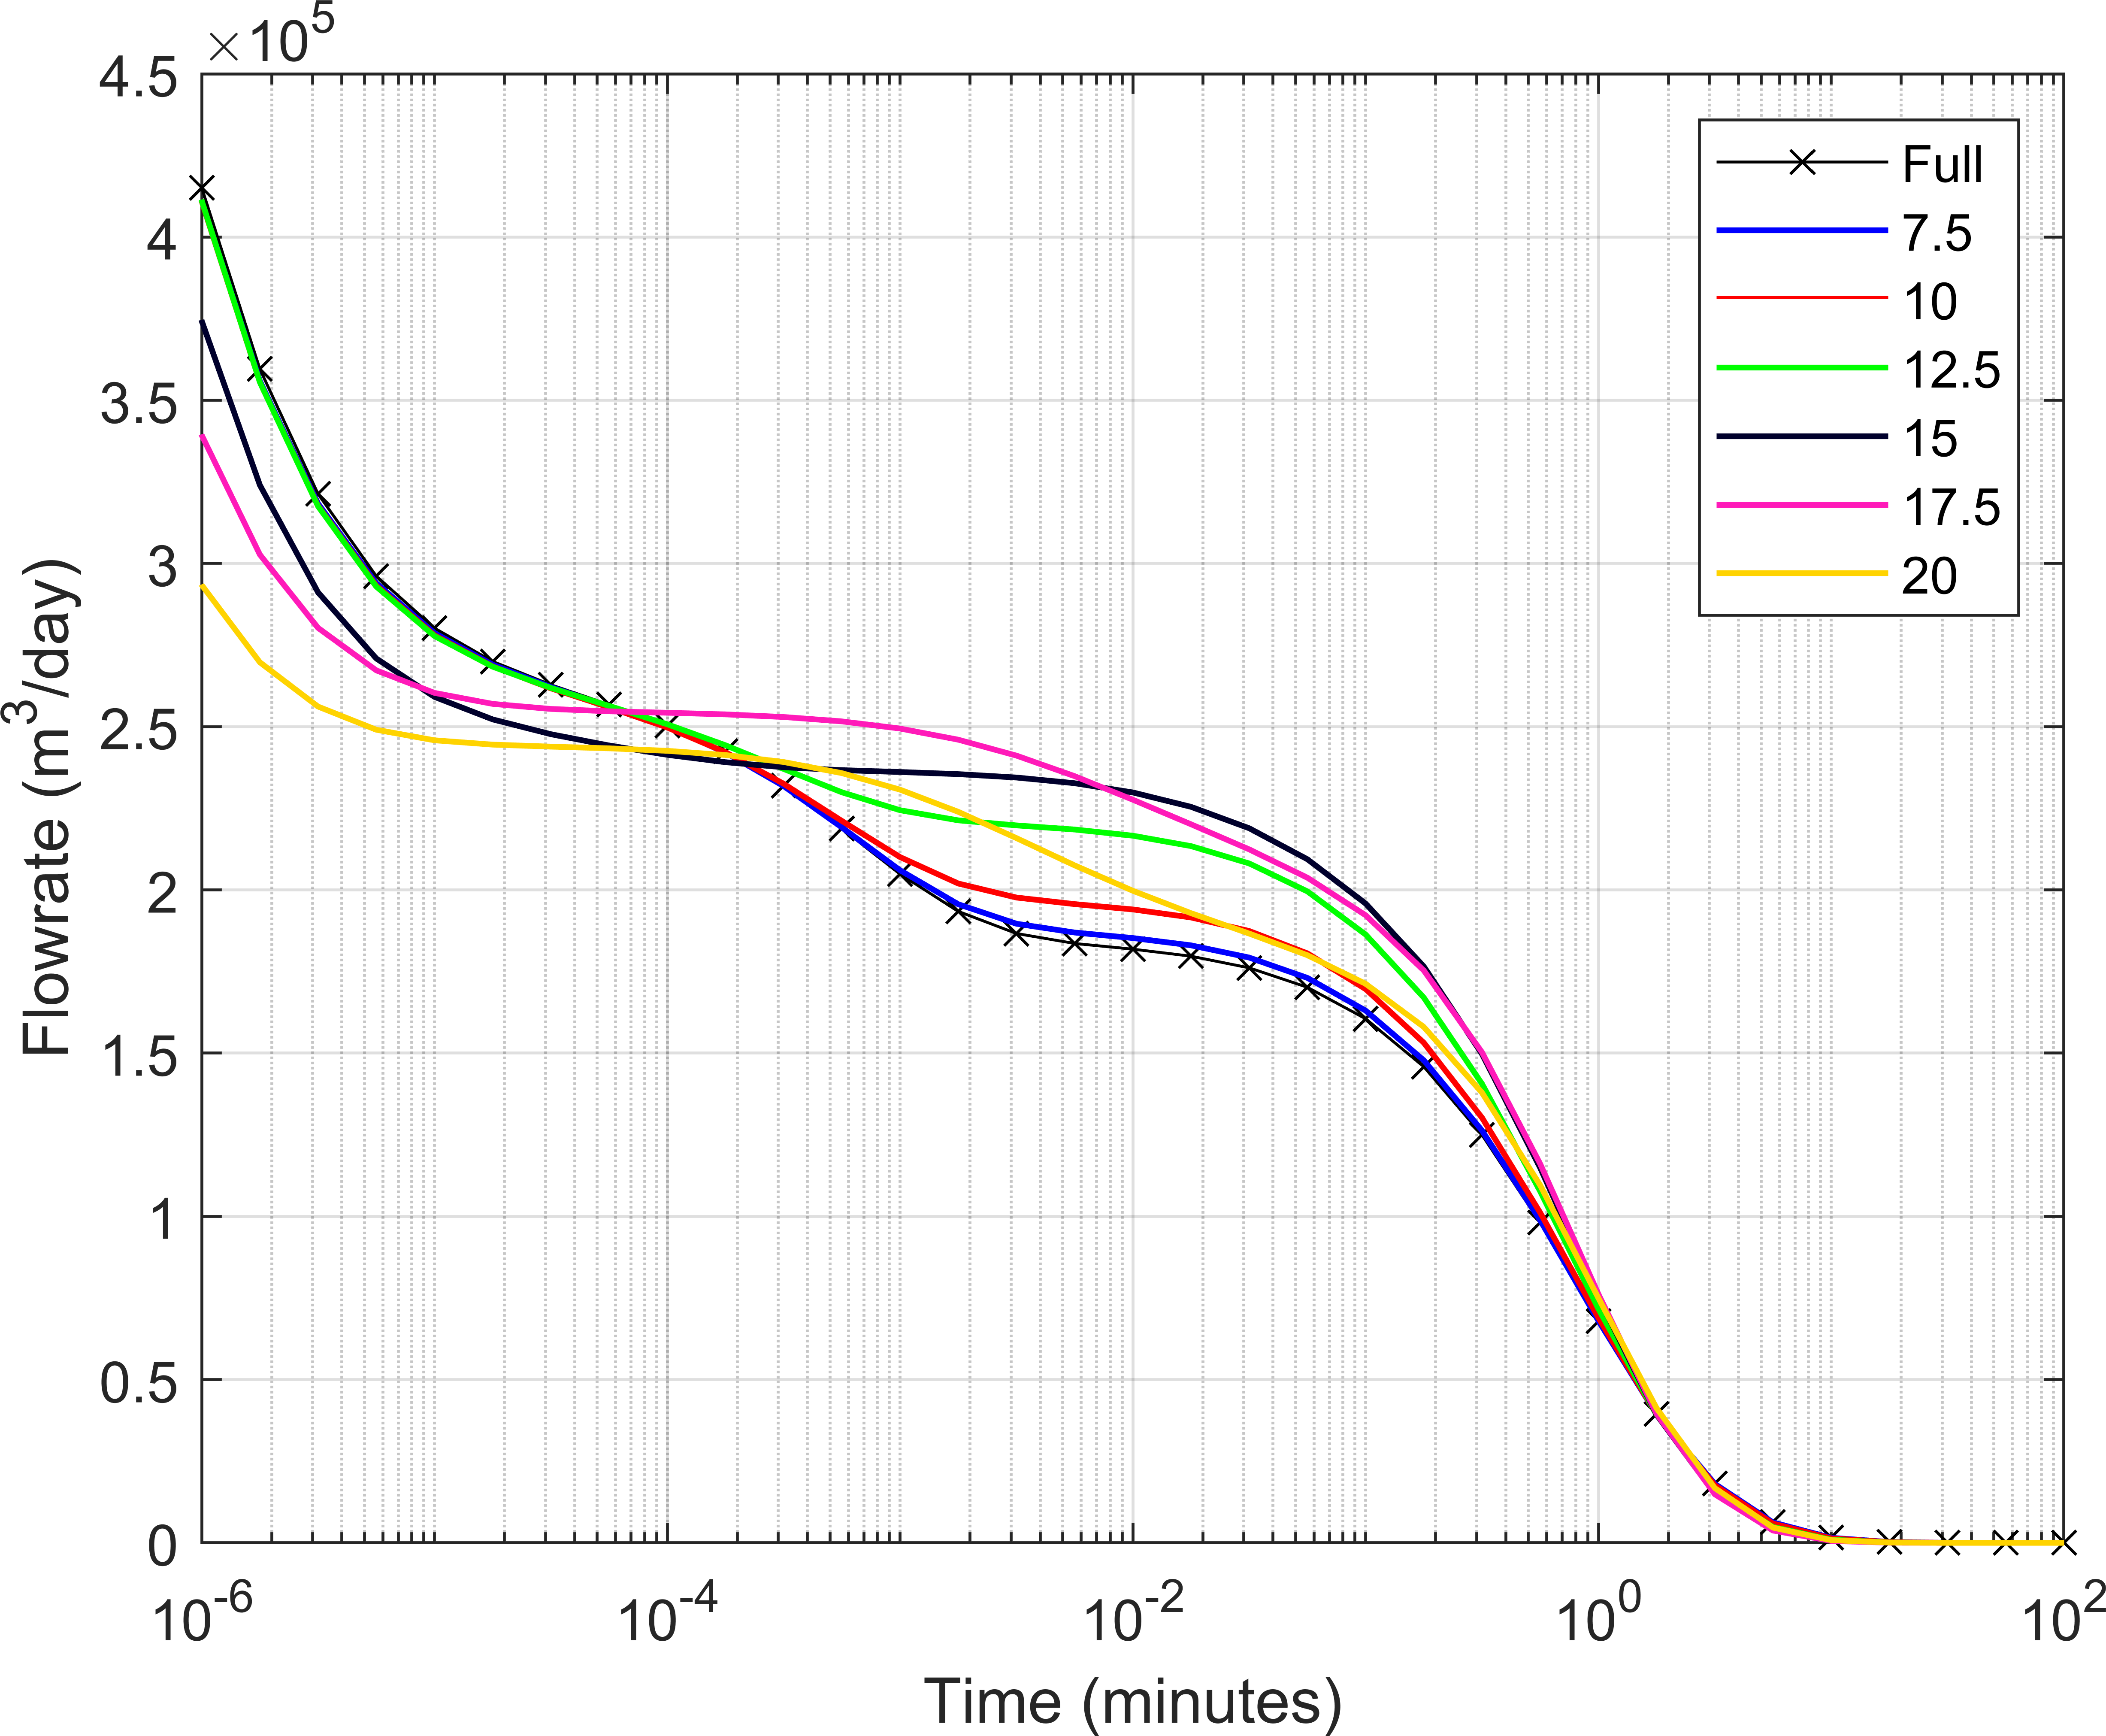
\includegraphics[width=\textwidth]{3D_DD/Plot_Drawdown_Case_09_nohead.png}
        \subcaption{Case 9}
        \label{fig:3D_DD_9}
     \end{subfigure}
     \\
     \begin{subfigure}{0.3\textwidth}
        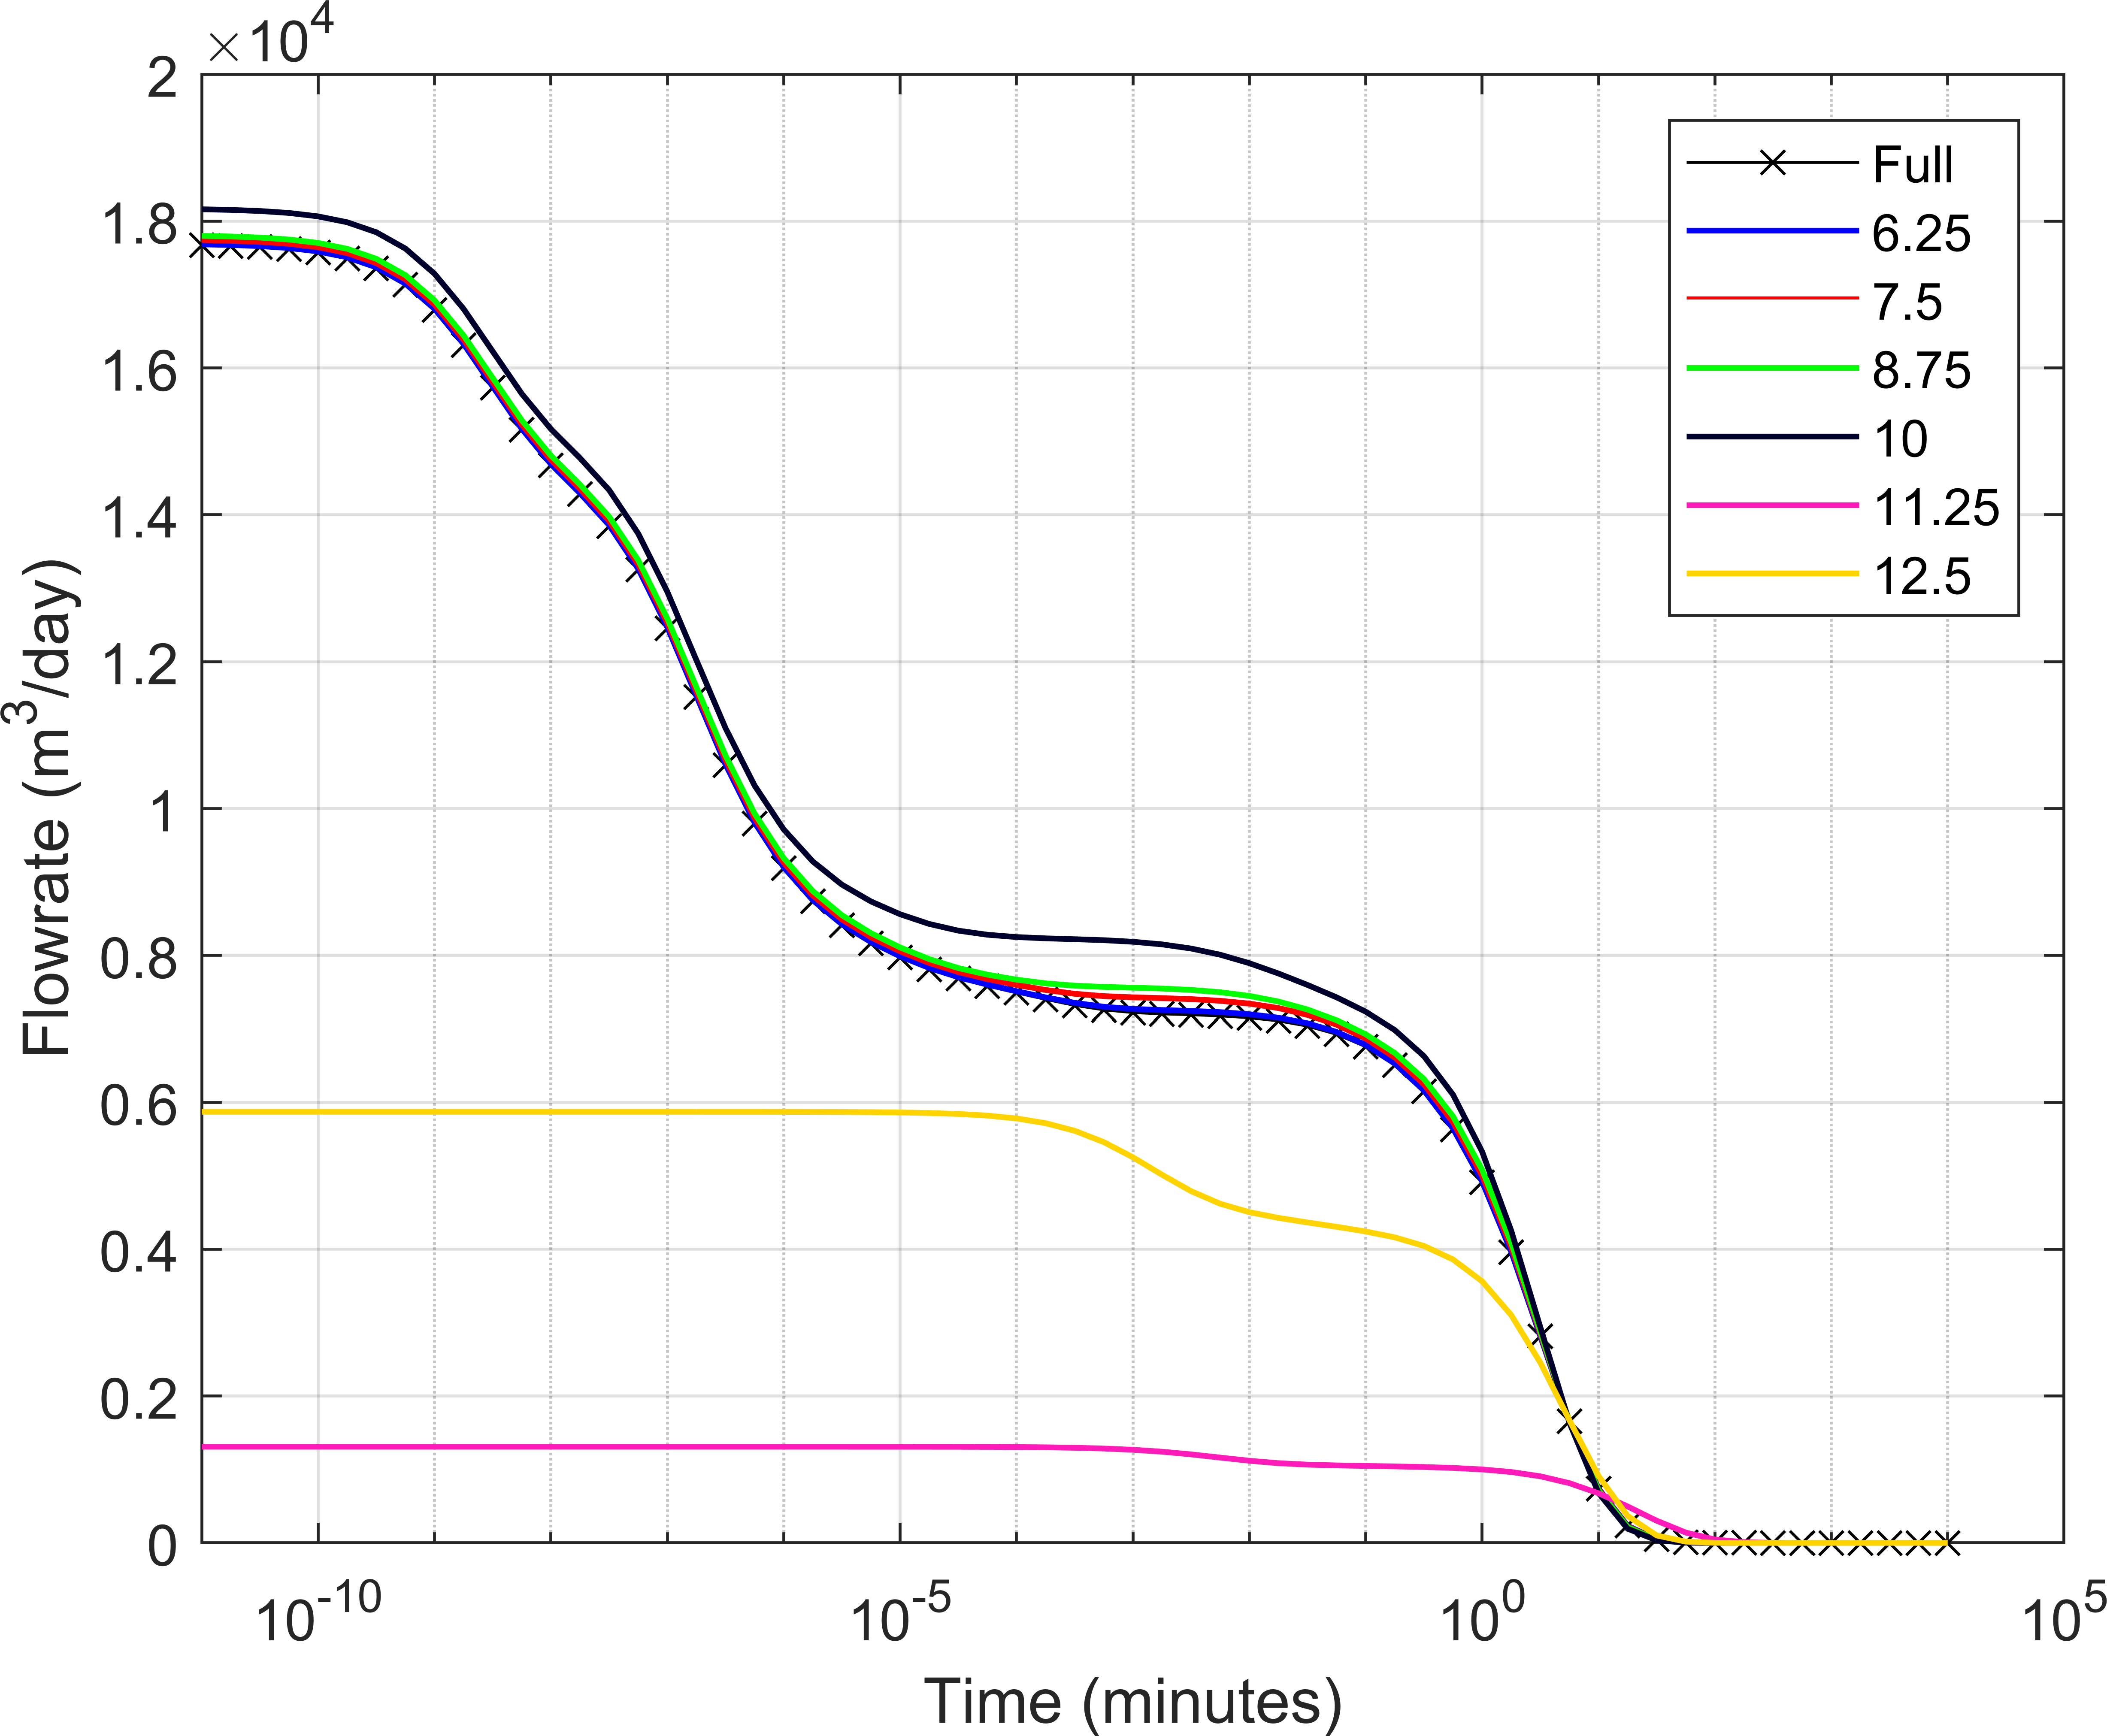
\includegraphics[width=\textwidth]{3D_DD/Plot_Drawdown_Case_10_nohead.png}
        \subcaption{Case 10}
        \label{fig:3D_DD_10}
     \end{subfigure}
     \begin{subfigure}{0.3\textwidth}
        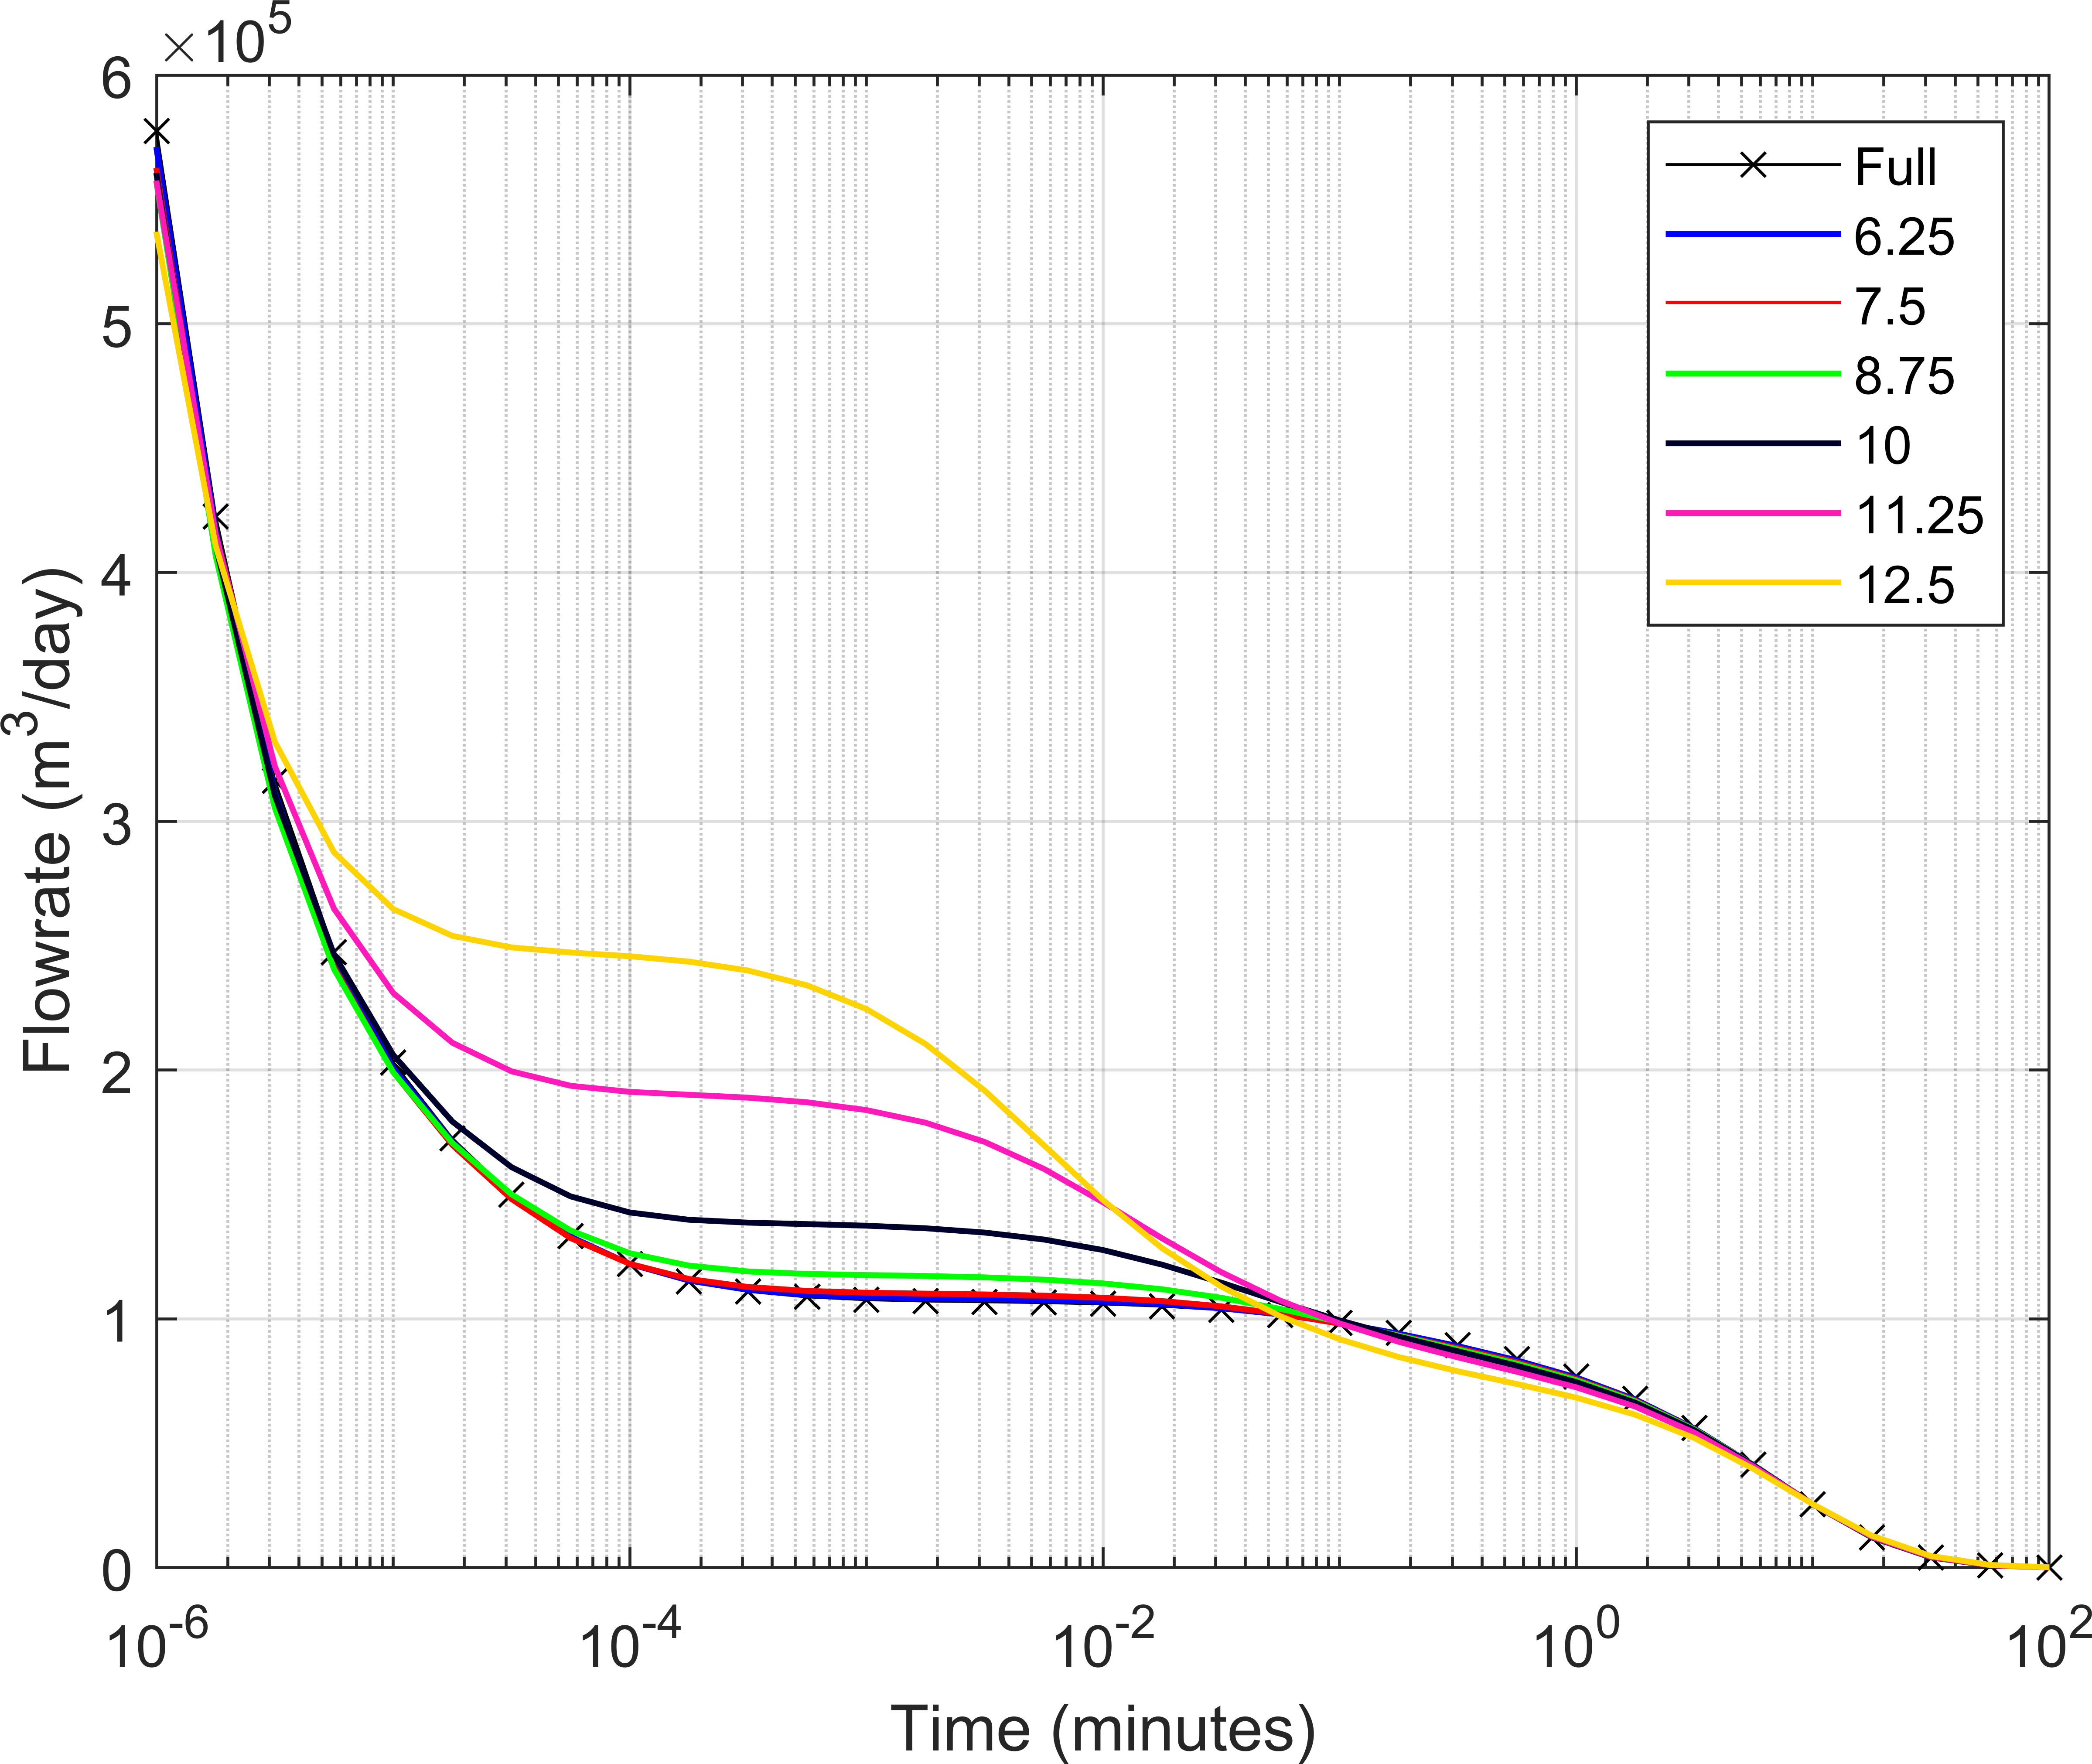
\includegraphics[width=\textwidth]{3D_DD/Plot_Drawdown_Case_11_nohead.png}
        \subcaption{Case 11}
        \label{fig:3D_DD_11}
     \end{subfigure}
     \begin{subfigure}{0.3\textwidth}
        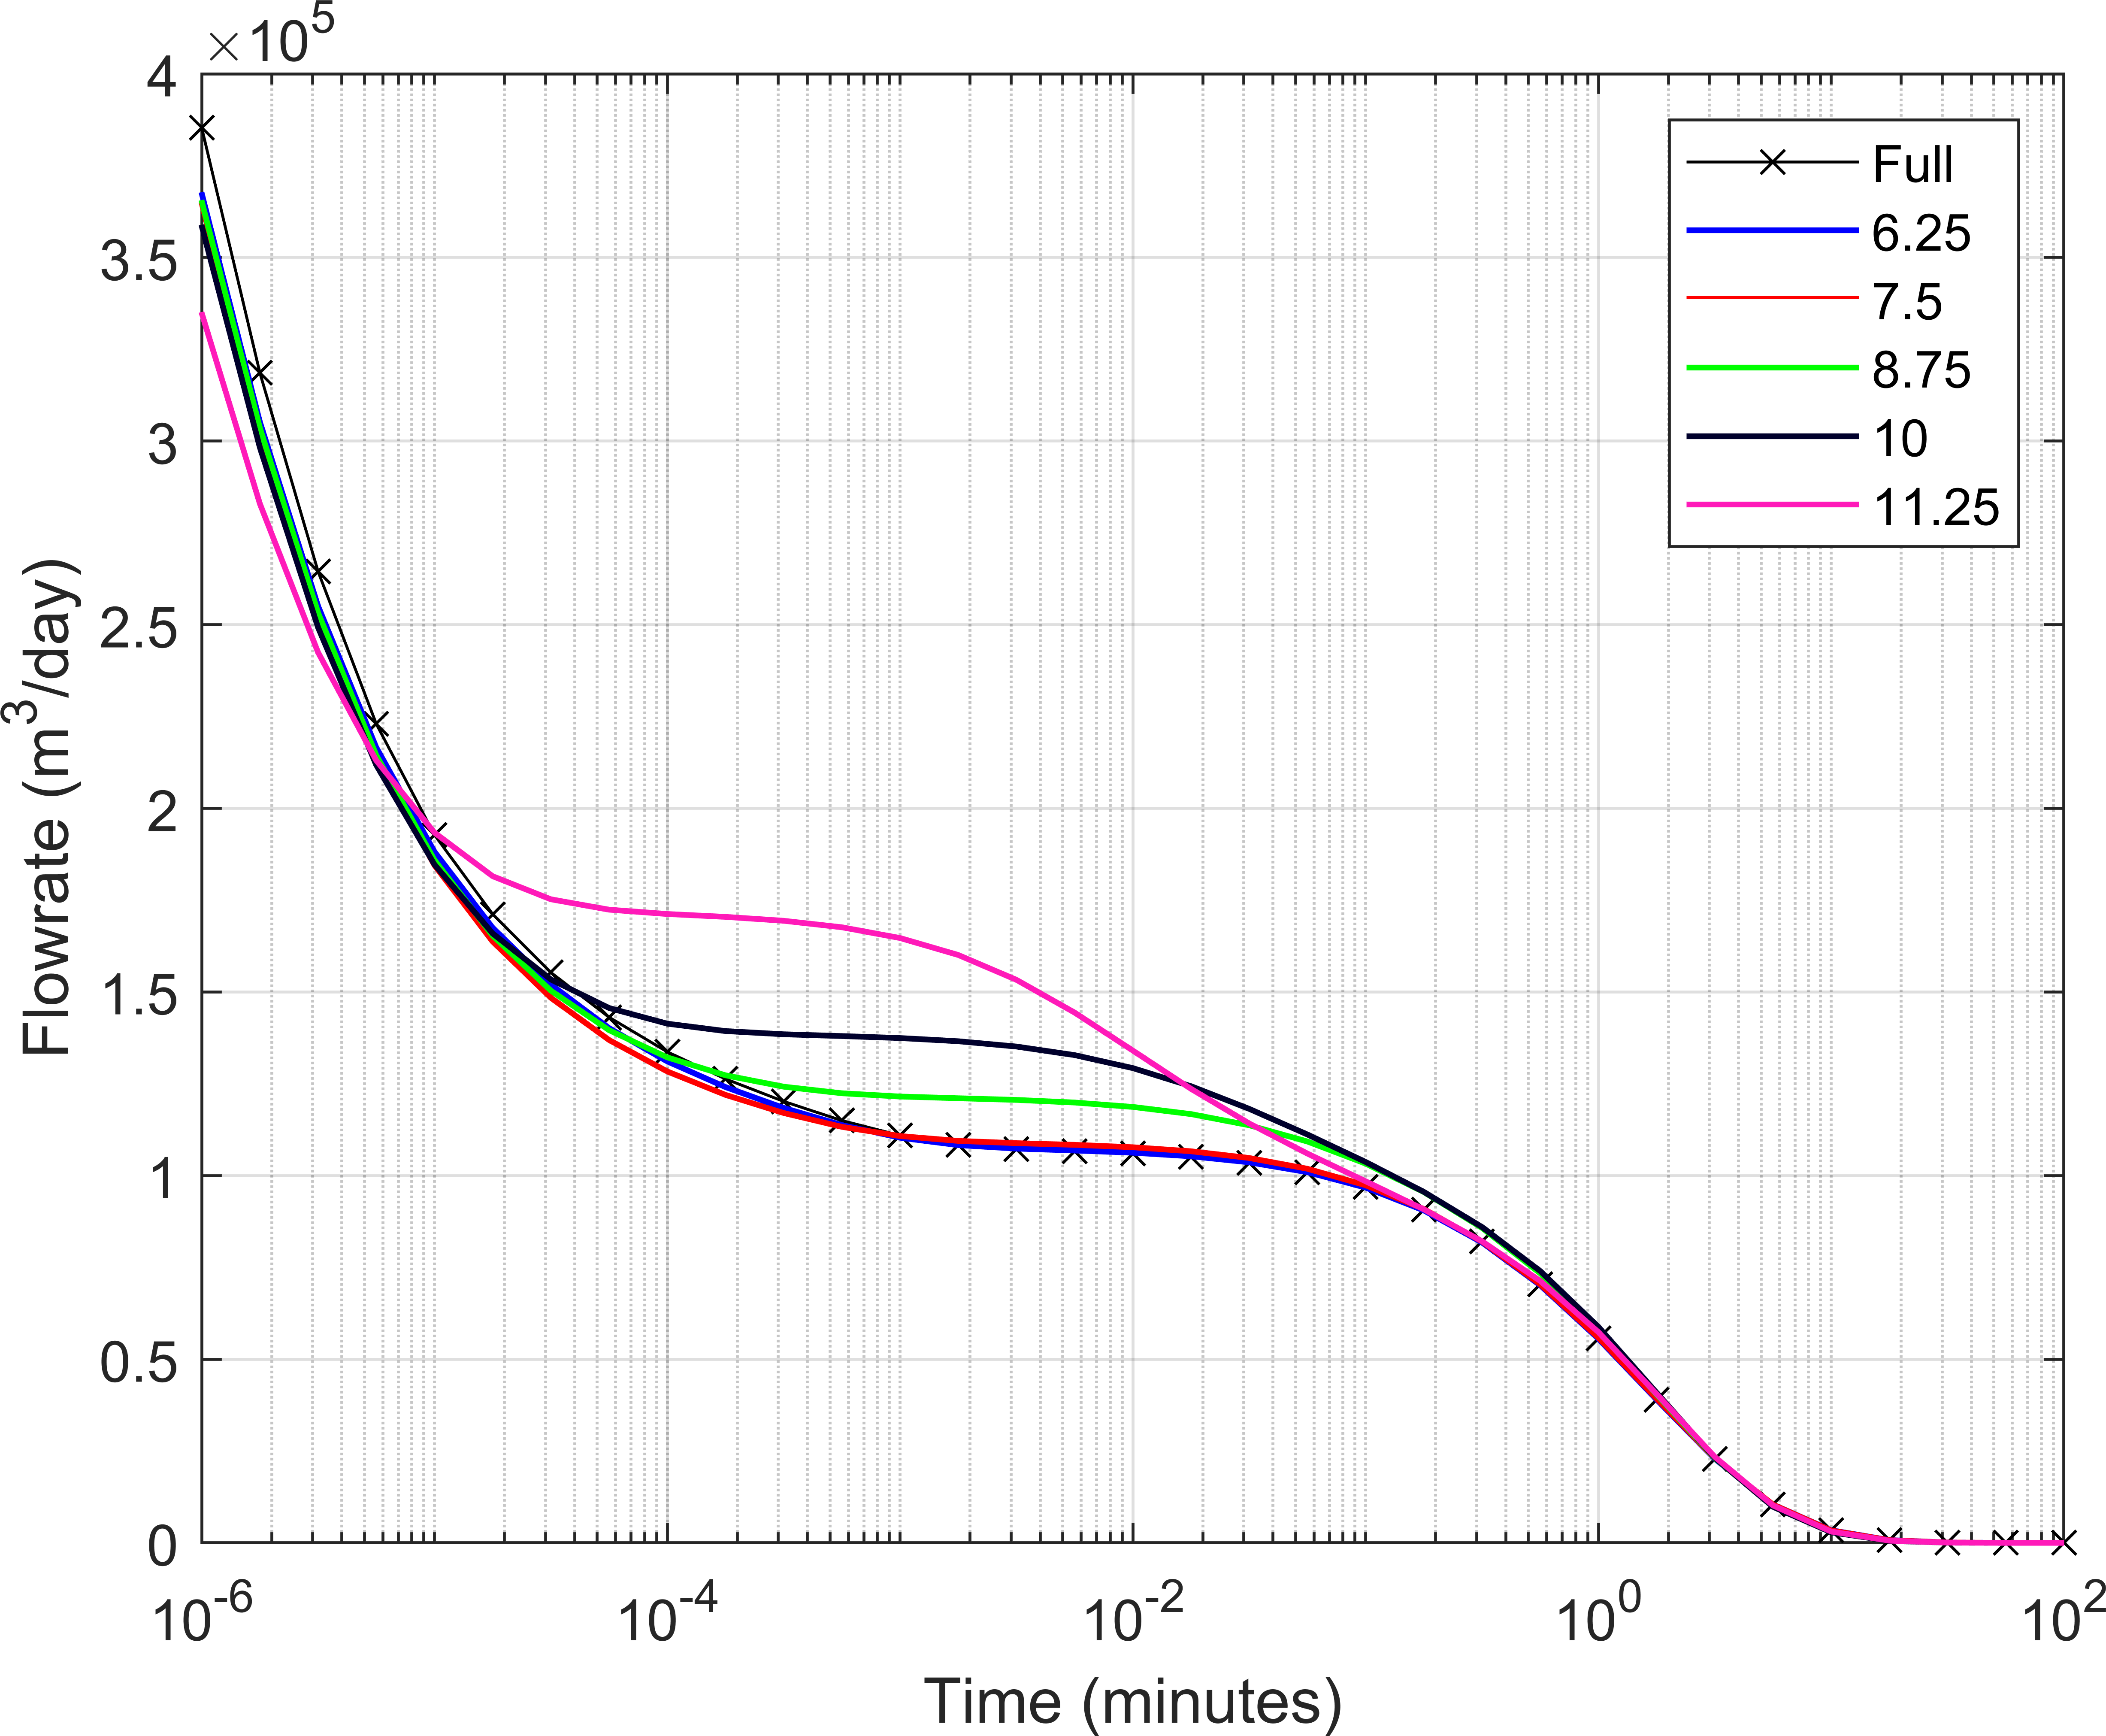
\includegraphics[width=\textwidth]{3D_DD/Plot_Drawdown_Case_12_nohead.png}
        \subcaption{Case 12}
        \label{fig:3D_DD_12}
     \end{subfigure}
     \\
     \begin{subfigure}{0.3\textwidth}
        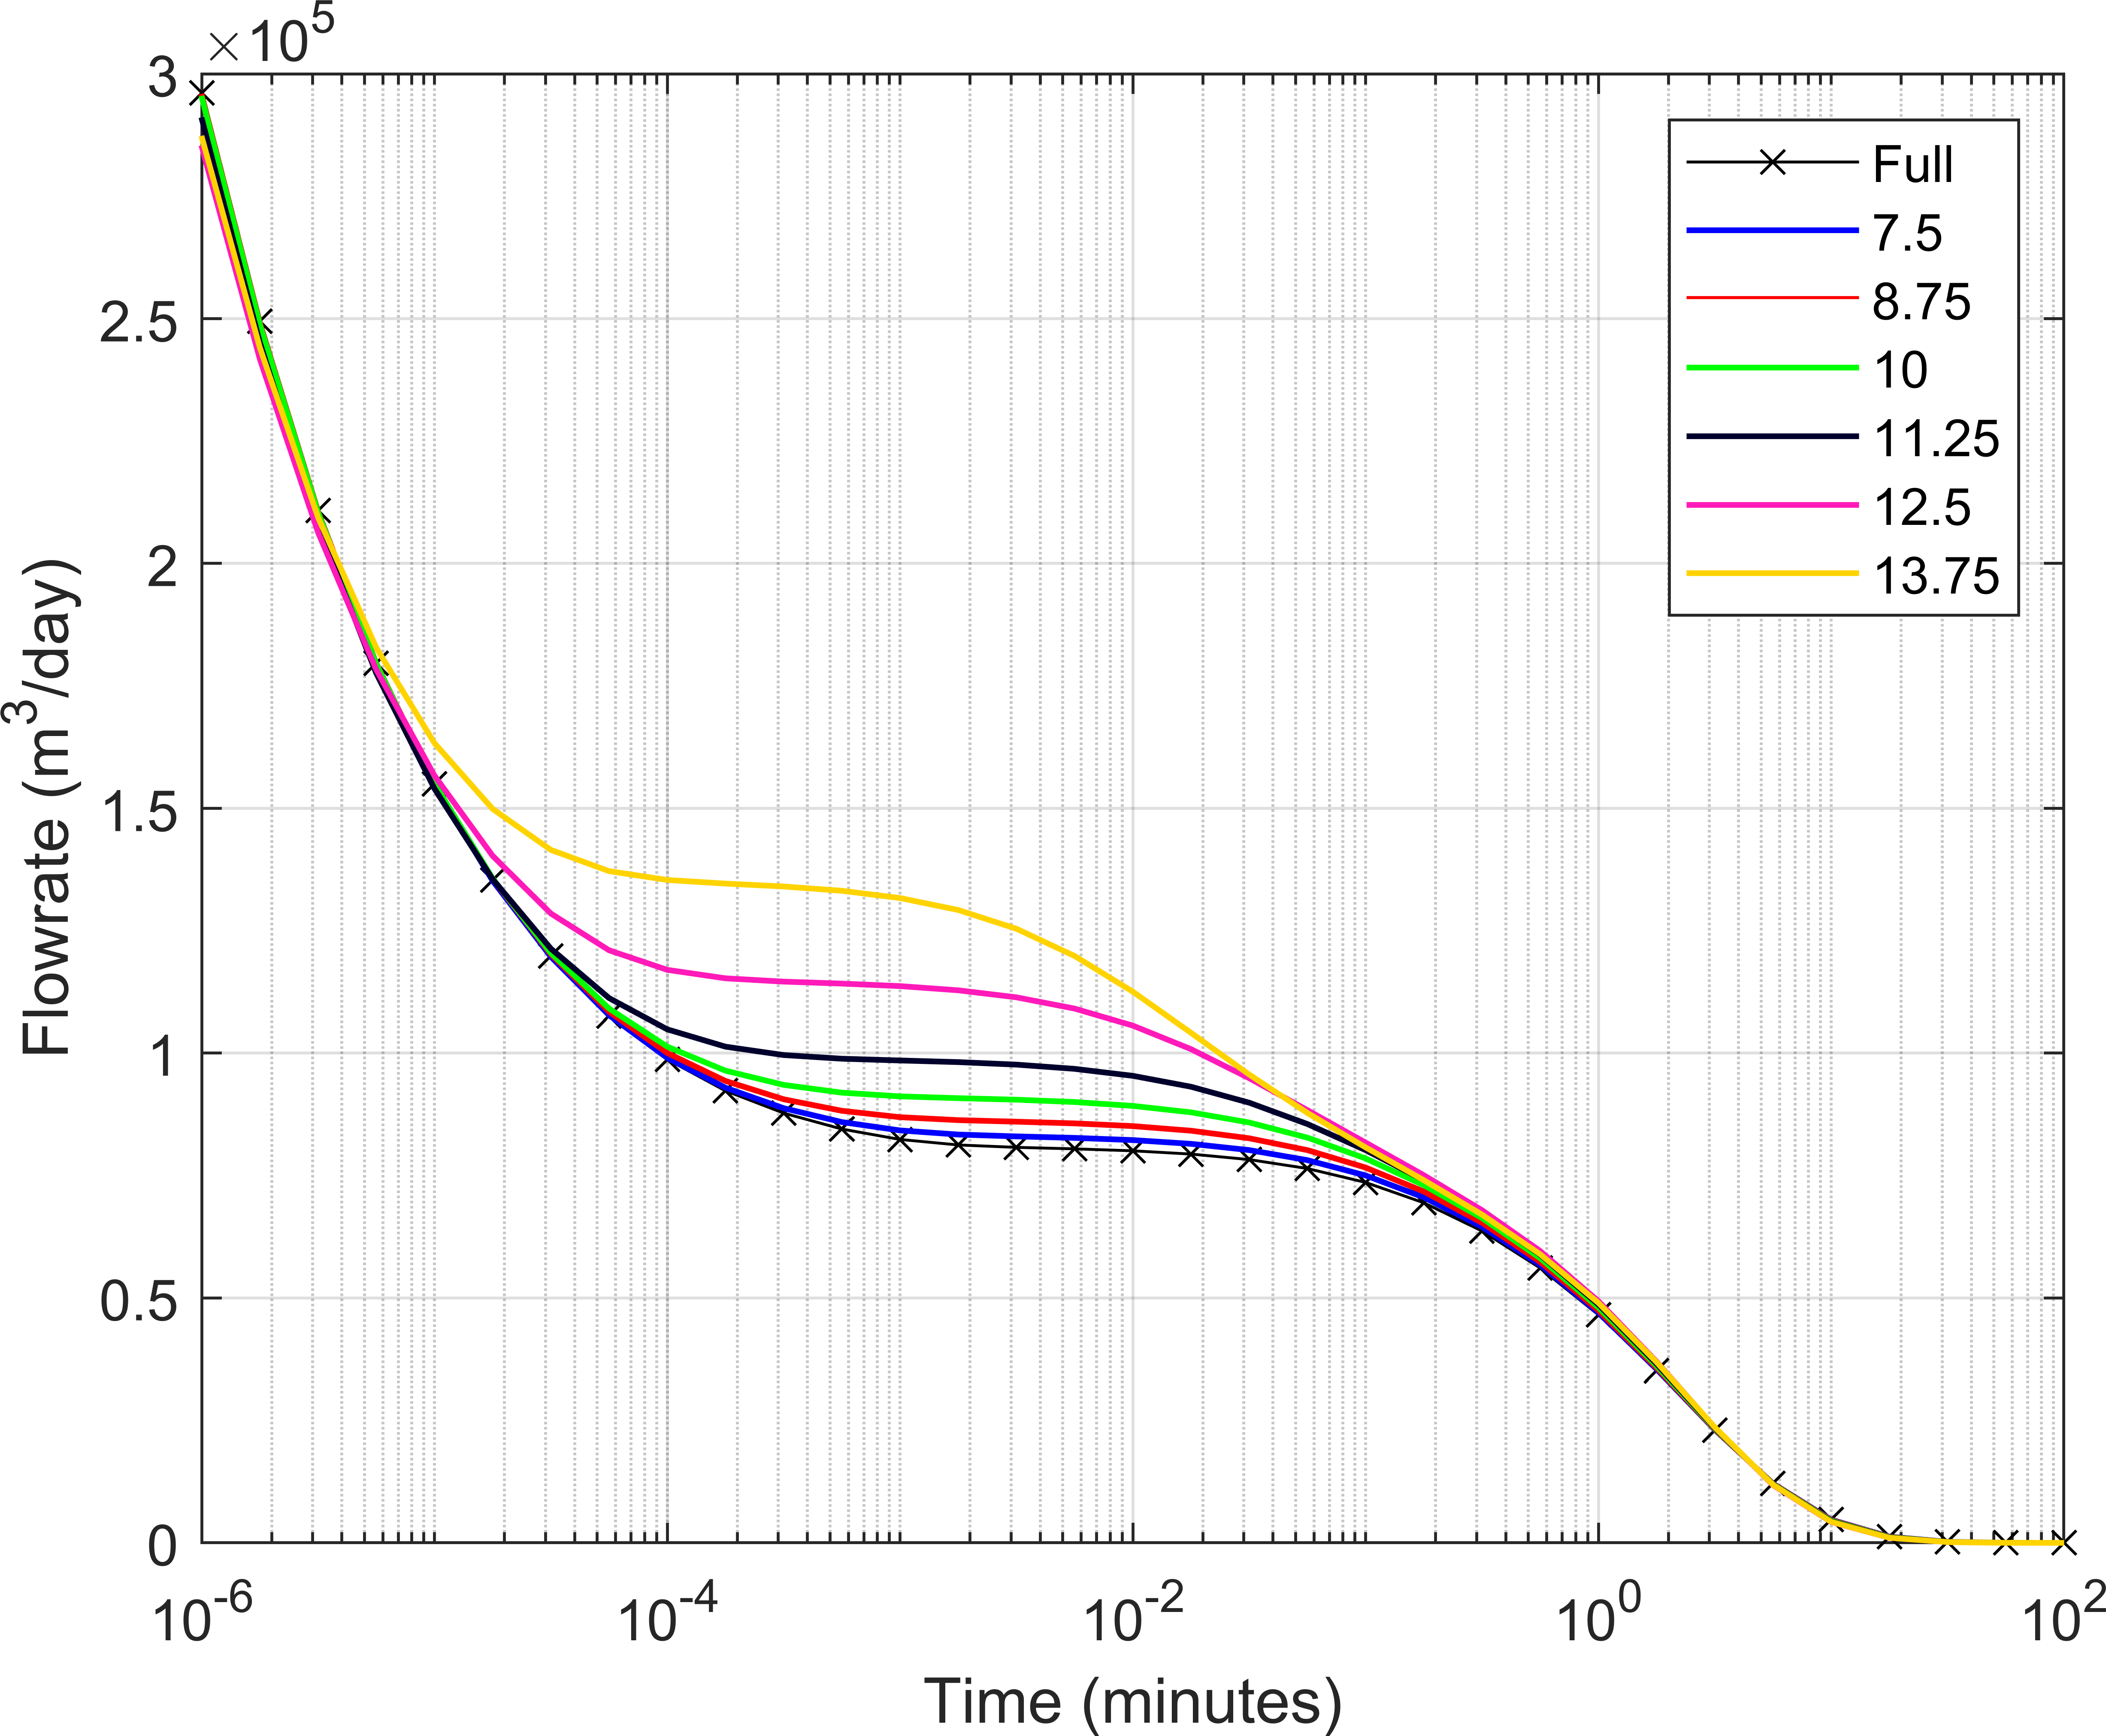
\includegraphics[width=\textwidth]{3D_DD/Plot_Drawdown_Case_13_nohead.png}
        \subcaption{Case 13}
        \label{fig:3D_DD_13}
     \end{subfigure}
     \begin{subfigure}{0.25\textwidth}
        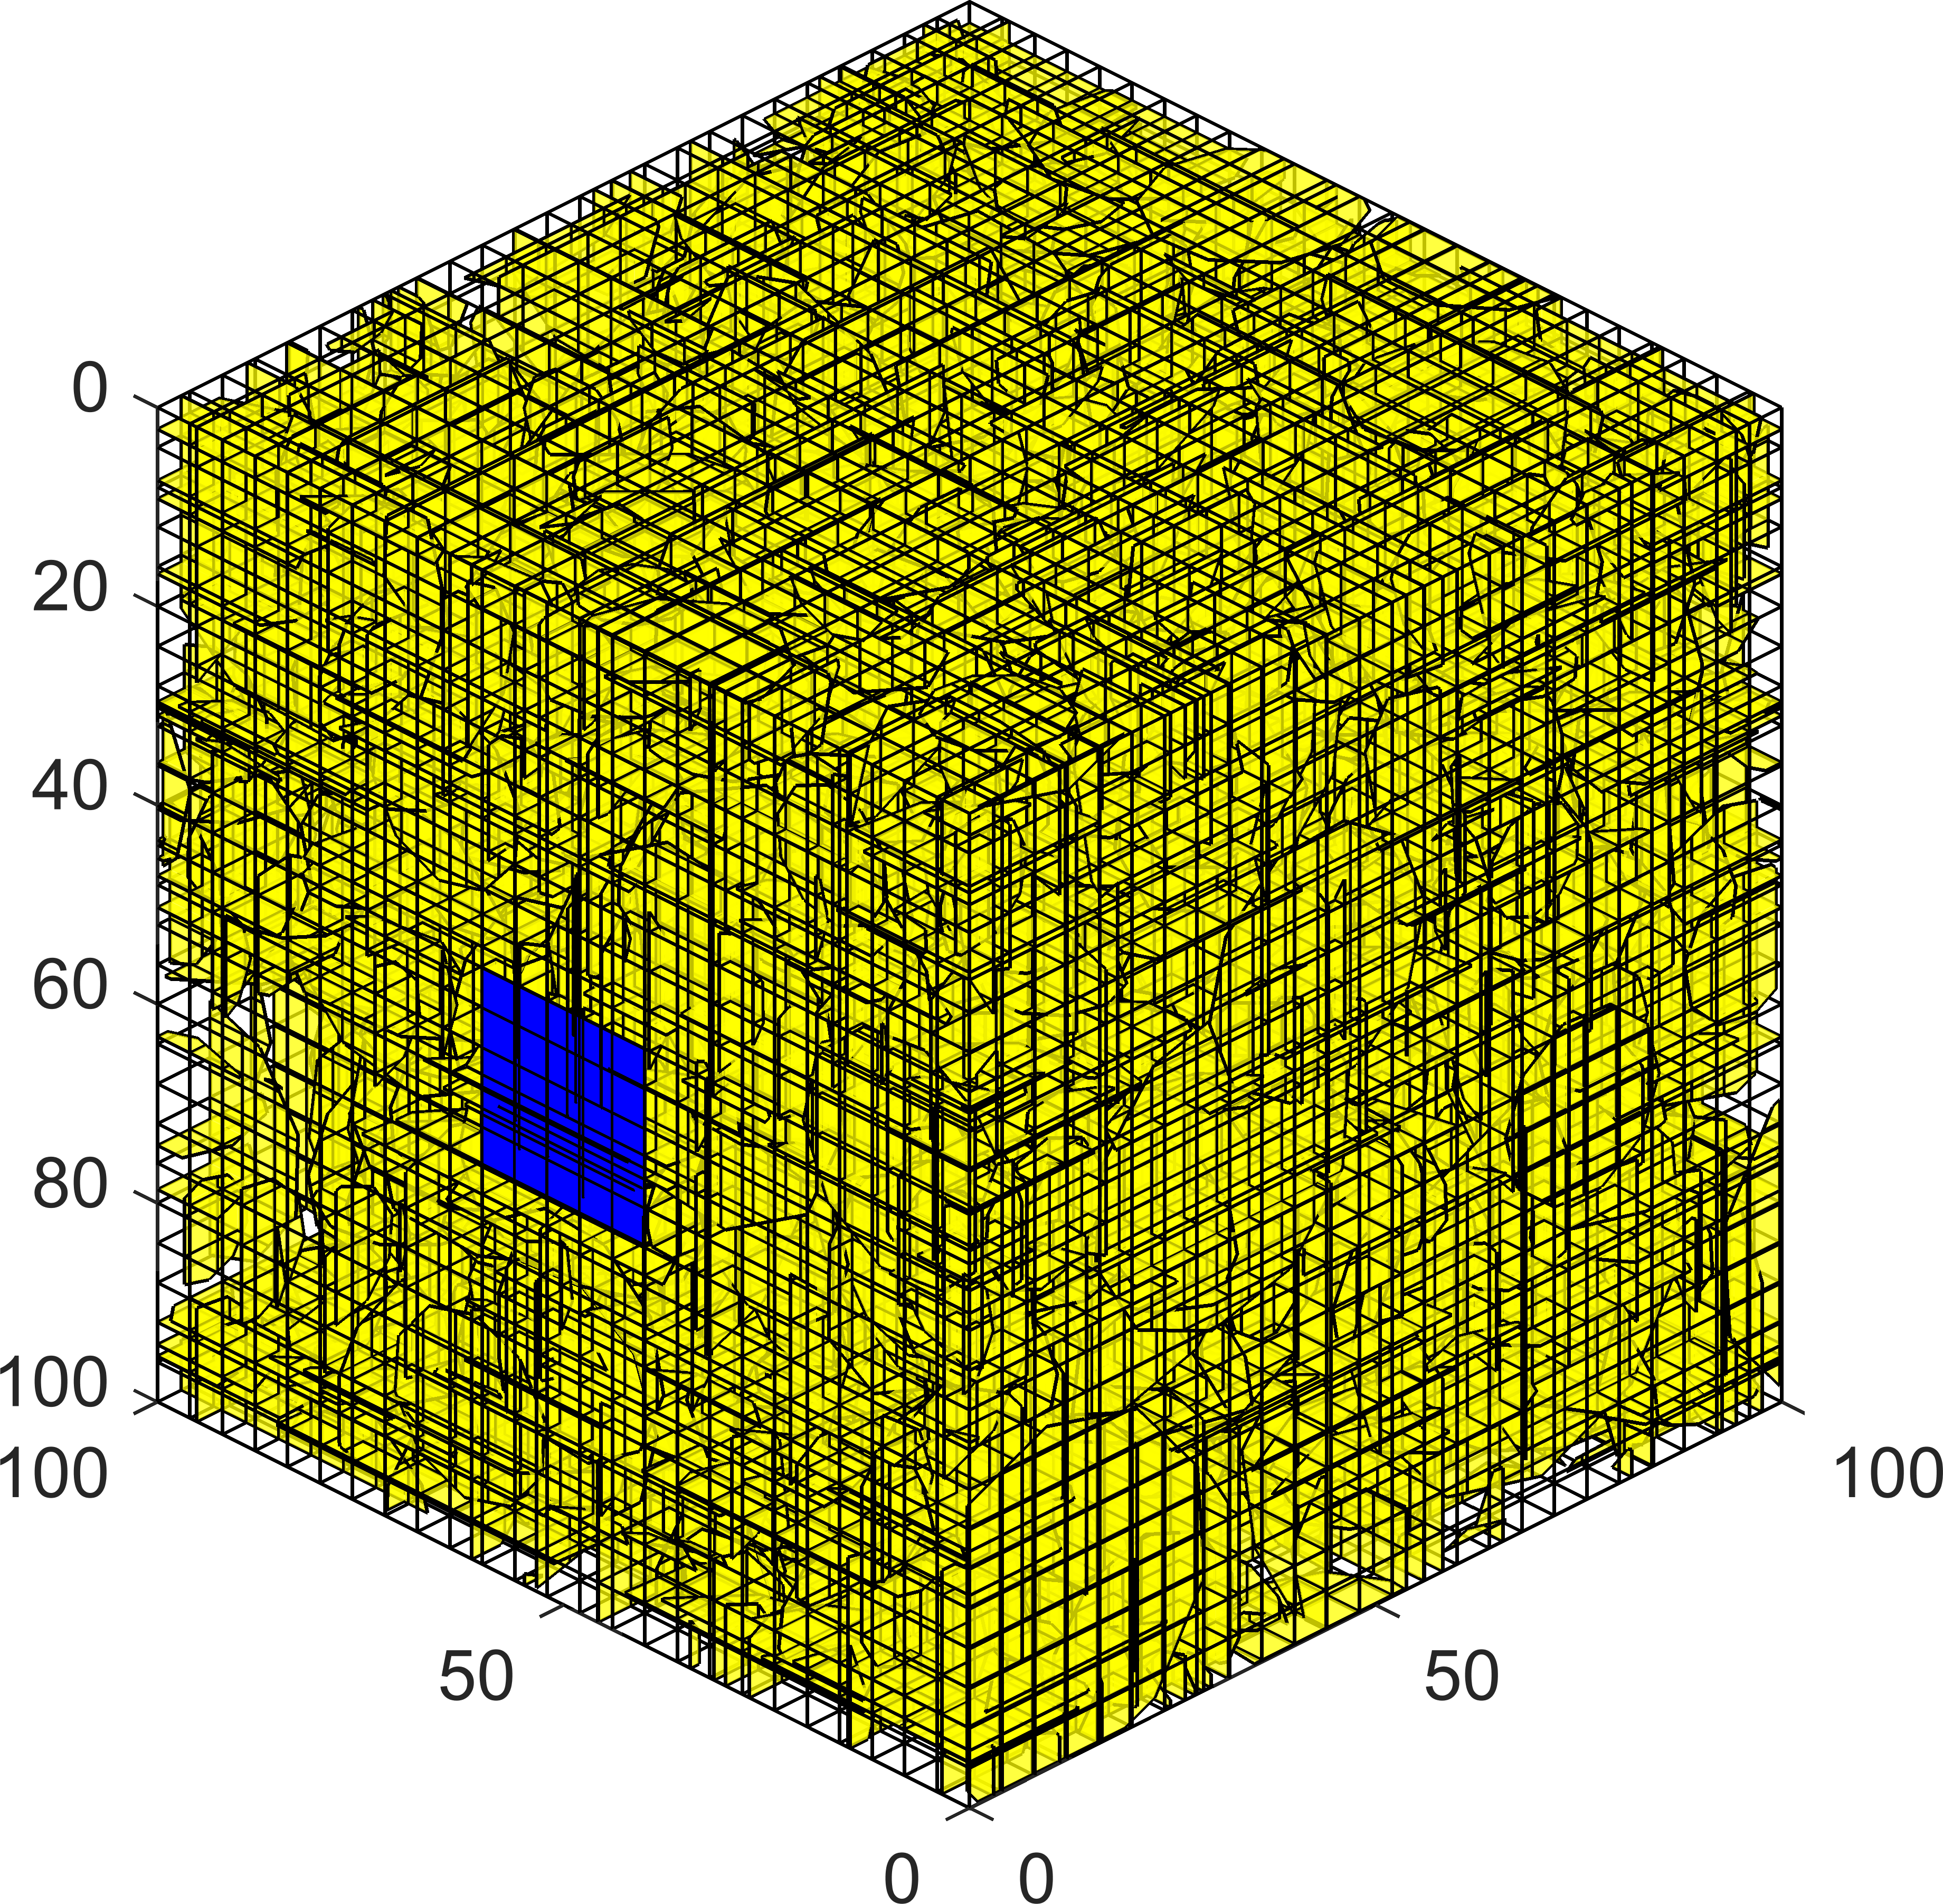
\includegraphics[width=\textwidth]{3D_DD/Boundarycondition.png}
        \subcaption{Boundary Condition}
        \label{fig:3D_BC}
     \end{subfigure}
     \caption{Pressure drawdown curves for 3D DFNs. (a)-(m) Full model solutions are compared to output from hybrid models created using various partitioning sizes (shown in legend). (n) A fixed pressure is applied on the blue faces for all simulations. Fractures are highlighted in yellow.}
     \label{fig:3D_DD}
 \end{figure}
\end{document}